
%% bare_jrnl.tex
%% V1.4b
%% 2015/08/26
%% by Michael Shell
%% see http://www.michaelshell.org/
%% for current contact information.
%%
%% This is a skeleton file demonstrating the use of IEEEtran.cls
%% (requires IEEEtran.cls version 1.8b or later) with an IEEE
%% journal paper.
%%
%% Support sites:
%% http://www.michaelshell.org/tex/ieeetran/
%% http://www.ctan.org/pkg/ieeetran
%% and
%% http://www.ieee.org/

%%*************************************************************************
%% Legal Notice:
%% This code is offered as-is without any warranty either expressed or
%% implied; without even the implied warranty of MERCHANTABILITY or
%% FITNESS FOR A PARTICULAR PURPOSE! 
%% User assumes all risk.
%% In no event shall the IEEE or any contributor to this code be liable for
%% any damages or losses, including, but not limited to, incidental,
%% consequential, or any other damages, resulting from the use or misuse
%% of any information contained here.
%%
%% All comments are the opinions of their respective authors and are not
%% necessarily endorsed by the IEEE.
%%
%% This work is distributed under the LaTeX Project Public License (LPPL)
%% ( http://www.latex-project.org/ ) version 1.3, and may be freely used,
%% distributed and modified. A copy of the LPPL, version 1.3, is included
%% in the base LaTeX documentation of all distributions of LaTeX released
%% 2003/12/01 or later.
%% Retain all contribution notices and credits.
%% ** Modified files should be clearly indicated as such, including  **
%% ** renaming them and changing author support contact information. **
%%*************************************************************************


% *** Authors should verify (and, if needed, correct) their LaTeX system  ***
% *** with the testflow diagnostic prior to trusting their LaTeX platform ***
% *** with production work. The IEEE's font choices and paper sizes can   ***
% *** trigger bugs that do not appear when using other class files.       ***                          ***
% The testflow support page is at:
% http://www.michaelshell.org/tex/testflow/



\documentclass[peerreview]{IEEEtran}
%
% If IEEEtran.cls has not been installed into the LaTeX system files,
% manually specify the path to it like:
% \documentclass[journal]{../sty/IEEEtran}





% Some very useful LaTeX packages include:
% (uncomment the ones you want to load)


% *** MISC UTILITY PACKAGES ***
%
%\usepackage{ifpdf}
% Heiko Oberdiek's ifpdf.sty is very useful if you need conditional
% compilation based on whether the output is pdf or dvi.
% usage:
% \ifpdf
%   % pdf code
% \else
%   % dvi code
% \fi
% The latest version of ifpdf.sty can be obtained from:
% http://www.ctan.org/pkg/ifpdf
% Also, note that IEEEtran.cls V1.7 and later provides a builtin
% \ifCLASSINFOpdf conditional that works the same way.
% When switching from latex to pdflatex and vice-versa, the compiler may
% have to be run twice to clear warning/error messages.






% *** CITATION PACKAGES ***
%
%\usepackage{cite}
% cite.sty was written by Donald Arseneau
% V1.6 and later of IEEEtran pre-defines the format of the cite.sty package
% \cite{} output to follow that of the IEEE. Loading the cite package will
% result in citation numbers being automatically sorted and properly
% "compressed/ranged". e.g., [1], [9], [2], [7], [5], [6] without using
% cite.sty will become [1], [2], [5]--[7], [9] using cite.sty. cite.sty's
% \cite will automatically add leading space, if needed. Use cite.sty's
% noadjust option (cite.sty V3.8 and later) if you want to turn this off
% such as if a citation ever needs to be enclosed in parenthesis.
% cite.sty is already installed on most LaTeX systems. Be sure and use
% version 5.0 (2009-03-20) and later if using hyperref.sty.
% The latest version can be obtained at:
% http://www.ctan.org/pkg/cite
% The documentation is contained in the cite.sty file itself.






% *** GRAPHICS RELATED PACKAGES ***
%
\ifCLASSINFOpdf
  % \usepackage[pdftex]{graphicx}
  % declare the path(s) where your graphic files are
  % \graphicspath{{../pdf/}{../jpeg/}}
  % and their extensions so you won't have to specify these with
  % every instance of \includegraphics
  % \DeclareGraphicsExtensions{.pdf,.jpeg,.png}
\else
  % or other class option (dvipsone, dvipdf, if not using dvips). graphicx
  % will default to the driver specified in the system graphics.cfg if no
  % driver is specified.
  % \usepackage[dvips]{graphicx}
  % declare the path(s) where your graphic files are
  % \graphicspath{{../eps/}}
  % and their extensions so you won't have to specify these with
  % every instance of \includegraphics
  % \DeclareGraphicsExtensions{.eps}
\fi
% graphicx was written by David Carlisle and Sebastian Rahtz. It is
% required if you want graphics, photos, etc. graphicx.sty is already
% installed on most LaTeX systems. The latest version and documentation
% can be obtained at: 
% http://www.ctan.org/pkg/graphicx
% Another good source of documentation is "Using Imported Graphics in
% LaTeX2e" by Keith Reckdahl which can be found at:
% http://www.ctan.org/pkg/epslatex
%
% latex, and pdflatex in dvi mode, support graphics in encapsulated
% postscript (.eps) format. pdflatex in pdf mode supports graphics
% in .pdf, .jpeg, .png and .mps (metapost) formats. Users should ensure
% that all non-photo figures use a vector format (.eps, .pdf, .mps) and
% not a bitmapped formats (.jpeg, .png). The IEEE frowns on bitmapped formats
% which can result in "jaggedy"/blurry rendering of lines and letters as
% well as large increases in file sizes.
%
% You can find documentation about the pdfTeX application at:
% http://www.tug.org/applications/pdftex





% *** MATH PACKAGES ***
%
%\usepackage{amsmath}
% A popular package from the American Mathematical Society that provides
% many useful and powerful commands for dealing with mathematics.
%
% Note that the amsmath package sets \interdisplaylinepenalty to 10000
% thus preventing page breaks from occurring within multiline equations. Use:
%\interdisplaylinepenalty=2500
% after loading amsmath to restore such page breaks as IEEEtran.cls normally
% does. amsmath.sty is already installed on most LaTeX systems. The latest
% version and documentation can be obtained at:
% http://www.ctan.org/pkg/amsmath





% *** SPECIALIZED LIST PACKAGES ***
%
%\usepackage{algorithmic}
% algorithmic.sty was written by Peter Williams and Rogerio Brito.
% This package provides an algorithmic environment fo describing algorithms.
% You can use the algorithmic environment in-text or within a figure
% environment to provide for a floating algorithm. Do NOT use the algorithm
% floating environment provided by algorithm.sty (by the same authors) or
% algorithm2e.sty (by Christophe Fiorio) as the IEEE does not use dedicated
% algorithm float types and packages that provide these will not provide
% correct IEEE style captions. The latest version and documentation of
% algorithmic.sty can be obtained at:
% http://www.ctan.org/pkg/algorithms
% Also of interest may be the (relatively newer and more customizable)
% algorithmicx.sty package by Szasz Janos:
% http://www.ctan.org/pkg/algorithmicx




% *** ALIGNMENT PACKAGES ***
%
%\usepackage{array}
% Frank Mittelbach's and David Carlisle's array.sty patches and improves
% the standard LaTeX2e array and tabular environments to provide better
% appearance and additional user controls. As the default LaTeX2e table
% generation code is lacking to the point of almost being broken with
% respect to the quality of the end results, all users are strongly
% advised to use an enhanced (at the very least that provided by array.sty)
% set of table tools. array.sty is already installed on most systems. The
% latest version and documentation can be obtained at:
% http://www.ctan.org/pkg/array


% IEEEtran contains the IEEEeqnarray family of commands that can be used to
% generate multiline equations as well as matrices, tables, etc., of high
% quality.




% *** SUBFIGURE PACKAGES ***
%\ifCLASSOPTIONcompsoc
%  \usepackage[caption=false,font=normalsize,labelfont=sf,textfont=sf]{subfig}
%\else
%  \usepackage[caption=false,font=footnotesize]{subfig}
%\fi
% subfig.sty, written by Steven Douglas Cochran, is the modern replacement
% for subfigure.sty, the latter of which is no longer maintained and is
% incompatible with some LaTeX packages including fixltx2e. However,
% subfig.sty requires and automatically loads Axel Sommerfeldt's caption.sty
% which will override IEEEtran.cls' handling of captions and this will result
% in non-IEEE style figure/table captions. To prevent this problem, be sure
% and invoke subfig.sty's "caption=false" package option (available since
% subfig.sty version 1.3, 2005/06/28) as this is will preserve IEEEtran.cls
% handling of captions.
% Note that the Computer Society format requires a larger sans serif font
% than the serif footnote size font used in traditional IEEE formatting
% and thus the need to invoke different subfig.sty package options depending
% on whether compsoc mode has been enabled.
%
% The latest version and documentation of subfig.sty can be obtained at:
% http://www.ctan.org/pkg/subfig




% *** FLOAT PACKAGES ***
%
%\usepackage{fixltx2e}
% fixltx2e, the successor to the earlier fix2col.sty, was written by
% Frank Mittelbach and David Carlisle. This package corrects a few problems
% in the LaTeX2e kernel, the most notable of which is that in current
% LaTeX2e releases, the ordering of single and double column floats is not
% guaranteed to be preserved. Thus, an unpatched LaTeX2e can allow a
% single column figure to be placed prior to an earlier double column
% figure.
% Be aware that LaTeX2e kernels dated 2015 and later have fixltx2e.sty's
% corrections already built into the system in which case a warning will
% be issued if an attempt is made to load fixltx2e.sty as it is no longer
% needed.
% The latest version and documentation can be found at:
% http://www.ctan.org/pkg/fixltx2e


%\usepackage{stfloats}
% stfloats.sty was written by Sigitas Tolusis. This package gives LaTeX2e
% the ability to do double column floats at the bottom of the page as well
% as the top. (e.g., "\begin{figure*}[!b]" is not normally possible in
% LaTeX2e). It also provides a command:
%\fnbelowfloat
% to enable the placement of footnotes below bottom floats (the standard
% LaTeX2e kernel puts them above bottom floats). This is an invasive package
% which rewrites many portions of the LaTeX2e float routines. It may not work
% with other packages that modify the LaTeX2e float routines. The latest
% version and documentation can be obtained at:
% http://www.ctan.org/pkg/stfloats
% Do not use the stfloats baselinefloat ability as the IEEE does not allow
% \baselineskip to stretch. Authors submitting work to the IEEE should note
% that the IEEE rarely uses double column equations and that authors should try
% to avoid such use. Do not be tempted to use the cuted.sty or midfloat.sty
% packages (also by Sigitas Tolusis) as the IEEE does not format its papers in
% such ways.
% Do not attempt to use stfloats with fixltx2e as they are incompatible.
% Instead, use Morten Hogholm'a dblfloatfix which combines the features
% of both fixltx2e and stfloats:
%
% \usepackage{dblfloatfix}
% The latest version can be found at:
% http://www.ctan.org/pkg/dblfloatfix




%\ifCLASSOPTIONcaptionsoff
%  \usepackage[nomarkers]{endfloat}
% \let\MYoriglatexcaption\caption
% \renewcommand{\caption}[2][\relax]{\MYoriglatexcaption[#2]{#2}}
%\fi
% endfloat.sty was written by James Darrell McCauley, Jeff Goldberg and 
% Axel Sommerfeldt. This package may be useful when used in conjunction with 
% IEEEtran.cls'  captionsoff option. Some IEEE journals/societies require that
% submissions have lists of figures/tables at the end of the paper and that
% figures/tables without any captions are placed on a page by themselves at
% the end of the document. If needed, the draftcls IEEEtran class option or
% \CLASSINPUTbaselinestretch interface can be used to increase the line
% spacing as well. Be sure and use the nomarkers option of endfloat to
% prevent endfloat from "marking" where the figures would have been placed
% in the text. The two hack lines of code above are a slight modification of
% that suggested by in the endfloat docs (section 8.4.1) to ensure that
% the full captions always appear in the list of figures/tables - even if
% the user used the short optional argument of \caption[]{}.
% IEEE papers do not typically make use of \caption[]'s optional argument,
% so this should not be an issue. A similar trick can be used to disable
% captions of packages such as subfig.sty that lack options to turn off
% the subcaptions:
% For subfig.sty:
% \let\MYorigsubfloat\subfloat
% \renewcommand{\subfloat}[2][\relax]{\MYorigsubfloat[]{#2}}
% However, the above trick will not work if both optional arguments of
% the \subfloat command are used. Furthermore, there needs to be a
% description of each subfigure *somewhere* and endfloat does not add
% subfigure captions to its list of figures. Thus, the best approach is to
% avoid the use of subfigure captions (many IEEE journals avoid them anyway)
% and instead reference/explain all the subfigures within the main caption.
% The latest version of endfloat.sty and its documentation can obtained at:
% http://www.ctan.org/pkg/endfloat
%
% The IEEEtran \ifCLASSOPTIONcaptionsoff conditional can also be used
% later in the document, say, to conditionally put the References on a 
% page by themselves.




% *** PDF, URL AND HYPERLINK PACKAGES ***
%
%\usepackage{url}
% url.sty was written by Donald Arseneau. It provides better support for
% handling and breaking URLs. url.sty is already installed on most LaTeX
% systems. The latest version and documentation can be obtained at:
% http://www.ctan.org/pkg/url
% Basically, \url{my_url_here}.




% *** Do not adjust lengths that control margins, column widths, etc. ***
% *** Do not use packages that alter fonts (such as pslatex).         ***
% There should be no need to do such things with IEEEtran.cls V1.6 and later.
% (Unless specifically asked to do so by the journal or conference you plan
% to submit to, of course. )


% correct bad hyphenation here
\hyphenation{op-tical net-works semi-conduc-tor}

\usepackage{amsmath}
\usepackage{caption}
\usepackage{subfig}
\usepackage{float}
\usepackage{booktabs}
\usepackage{tabularx}
\usepackage{tikz}
\usepackage{subfig}
\usepackage{adjustbox}
\usepackage[figuresright]{rotating}
\usepackage{tikz}
\usepackage{multirow}
\usepackage[hidelinks]{hyperref}
\usepackage{makecell}
\usepackage{calc}  % for '\widthof' macro
\usepackage{array} % for 'w' column type
\newlength\myleneiler
\newlength\mylenomega
\usetikzlibrary{shapes,arrows}
\tikzstyle{block} = [rectangle, draw, text width=4.5em, text centered, minimum height=4em]
\tikzstyle{line} = [draw, -latex']
\tikzstyle{decision} = [diamond, draw, text width=4.5em, text centered, inner sep=0pt]
\tikzstyle{cloud} = [draw, ellipse, text width=4.5em, text centered, minimum height=4em]
\usetikzlibrary{shapes, arrows.meta, positioning}
\tikzstyle{startstop} = [rectangle, rounded corners, minimum width=3cm, minimum height=1cm,text centered, draw=black, fill=red!30]
\tikzstyle{io} = [trapezium, trapezium left angle=70, trapezium right angle=110, minimum width=3cm, minimum height=1cm, text centered, draw=black, fill=blue!30]
\tikzstyle{process} = [rectangle, minimum width=3cm, minimum height=1cm, text centered, draw=black, fill=orange!30]
\tikzstyle{decision} = [diamond, minimum width=3cm, minimum height=1cm, text centered, draw=black, fill=green!30]
\tikzstyle{arrow} = [thick,->,>=stealth]
\setlength\myleneiler{(\widthof{Initial Condition (deg)}-4\tabcolsep)/3}
\setlength\mylenomega{(\widthof{Rotational Velocity Commands (rpm)}-4\tabcolsep)/4}


\begin{document}
%
% paper title
% Titles are generally capitalized except for words such as a, an, and, as,
% at, but, by, for, in, nor, of, on, or, the, to and up, which are usually
% not capitalized unless they are the first or last word of the title.
% Linebreaks \\ can be used within to get better formatting as desired.
% Do not put math or special symbols in the title.
\title{Attitude Control of a 3-DoF Quadrotor Platform using a Linear Quadratic Integral Differential Game Approach}
%
%
% author names and IEEE memberships
% note positions of commas and nonbreaking spaces ( ~ ) LaTeX will not break
% a structure at a ~ so this keeps an author's name from being broken across
% two lines.
% use \thanks{} to gain access to the first footnote area
% a separate \thanks must be used for each paragraph as LaTeX2e's \thanks
% was not built to handle multiple paragraphs
%

\author{Ali~Baniasad,~ Alireza Sharifi,~
        Reza~Pordal,~ Hadi~Nobahari
        % <-this % stops a space
}
% \thanks{M. Shell was with the Department
% of Electrical and Computer Engineering, Georgia Institute of Technology, Atlanta,
% GA, 30332 USA e-mail: (see http://www.michaelshell.org/contact.html).}% <-this % stops a space
% \thanks{J. Doe and J. Doe are with Anonymous University.}% <-this % stops a space
% \thanks{Manuscript received April 19, 2005; revised August 26, 2015.}}

% note the % following the last \IEEEmembership and also \thanks - 
% these prevent an unwanted space from occurring between the last author name
% and the end of the author line. i.e., if you had this:
% 
% \author{....lastname \thanks{...} \thanks{...} }
%                     ^------------^------------^----Do not want these spaces!
%
% a space would be appended to the last name and could cause every name on that
% line to be shifted left slightly. This is one of those "LaTeX things". For
% instance, "\textbf{A} \textbf{B}" will typeset as "A B" not "AB". To get
% "AB" then you have to do: "\textbf{A}\textbf{B}"
% \thanks is no different in this regard, so shield the last } of each \thanks
% that ends a line with a % and do not let a space in before the next \thanks.
% Spaces after \IEEEmembership other than the last one are OK (and needed) as
% you are supposed to have spaces between the names. For what it is worth,
% this is a minor point as most people would not even notice if the said evil
% space somehow managed to creep in.



% The paper headers
% \markboth{Journal of \LaTeX\ Class Files,~Vol.~14, No.~8, August~2015}% %%%?
% {Shell \MakeLowercase{\textit{et al.}}: Bare Demo of IEEEtran.cls for IEEE Journals} %%%?
% The only time the second header will appear is for the odd numbered pages
% after the title page when using the twoside option.
% 
% *** Note that you probably will NOT want to include the author's ***
% *** name in the headers of peer review papers.                   ***
% You can use \ifCLASSOPTIONpeerreview for conditional compilation here if
% you desire.




% If you want to put a publisher's ID mark on the page you can do it like
% this:
%\IEEEpubid{0000--0000/00\$00.00~\copyright~2015 IEEE}
% Remember, if you use this you must call \IEEEpubidadjcol in the second
% column for its text to clear the IEEEpubid mark.



% use for special paper notices
%\IEEEspecialpapernotice{(Invited Paper)}




% make the title area
\maketitle

\IEEEpeerreviewmaketitle

% As a general rule, do not put math, special symbols or citations
% in the abstract or keywords.
\begin{abstract}
  In this study, a linear quadratic integral differential game approach is applied to regulate and track the Euler angles for a quadrotor experimental platform using two players.
	One produces commands for each channel of the quadrotor and
	another generates the worst disturbance based on the mini-maximization of a quadratic criterion with integral action.
	For this purpose, first, the attitude dynamics of the platform are modeled and its parameters are identified based on the Nonlinear Least Squares Trust-Region Reflective method.
	The performance of the proposed controller is evaluated for regulation and tracking problems.
	The ability of the controller is also examined in the disturbance rejection.
	Moreover, the influence of uncertainty modeling is studied on the obtained results.
	Then, performance of the proposed controller is compared with the classic Proportional Integral Derivative, Linear Quadratic Regulator, and Linear Quadratic Integral Regulator. The results demonstrate the effectiveness of the Game Theory on the Linear Quadratic Regulator approach when the input disturbance occurs.
\end{abstract}

% Note that keywords are not normally used for peerreview papers.
\begin{IEEEkeywords}
  Linear Quadratic controller, Differential Game Theory, Quadrotor, 3-DoF Experimental Platform, Attitude Control. 
\end{IEEEkeywords}








% For peer review papers, you can put extra information on the cover
% page as needed:
% \ifCLASSOPTIONpeerreview
% \begin{center} \bfseries EDICS Category: 3-BBND \end{center}
% \fi
%
% For peerreview papers, this IEEEtran command inserts a page break and
% creates the second title. It will be ignored for other modes.
% \IEEEpeerreviewmaketitle



\section{Introduction}\label{sec:intro}
% The very first letter is a 2 line initial drop letter followed
% by the rest of the first word in caps.
% 
% form to use if the first word consists of a single letter:
% \IEEEPARstart{A}{demo} file is ....
% 
% form to use if you need the single drop letter followed by
% normal text (unknown if ever used by the IEEE):
% \IEEEPARstart{A}{}demo file is ....
% 
% Some journals put the first two words in caps:
% \IEEEPARstart{T}{his demo} file is ....
% 
% Here we have the typical use of a "T" for an initial drop letter
% and "HIS" in caps to complete the first word.
\IEEEPARstart{Q}{uadrotors}
are a type of Vertical Unmanned Aerial Vehicle (VUAV), that have various applications such as investigation, strategic operation, optical sensing, and entertainment.
The safe flight of the quadrotor in the presence of disturbances relies on precise control. 
A crucial subsystem of a control system for the quadrotor is the Attitude Control System (ACS). 
To regulate the quadrotor attitude, a Proportional Integral Derivative (PID) controller is utilized in \cite{article_Abdul, article_Bolandi}. Due to the nonlinearity dynamics of the quadrotor, the PID strategy is not effective in the presence of disturbance and modeling error.
To provide a faster control command in facing the modeling error and reduce the disturbance effect in the attitude control, the model-based control strategies including nonlinear control, intelligent control, optimal control, and robust control have been implemented on the ACS of the quadrotor.


Synergetic Control \cite{article_Chara}, Feedback Linearization (FBL) \cite{article_Aboudonia}, and Sliding Mode Control (SMC) \cite{7007285}, which are a group of the nonlinear control category, have been utilized to regulate the Euler angles (roll, pitch, and yaw angles) of the quadrotor. To control the attitude of the quadrotor intelligently, the controller strategies such as reinforcement learning \cite{LIN2020135}, iterative learning \cite{electronics10202474}, machine learning \cite{4564736} \cite{10007918}, and fuzzy logic \cite{KIM20211888} have been implemented. Moreover, to produce the optimal control commands, the controller strategies including Linear Quadratic Gaussian (LQG) \cite{7367782}, Linear Quadratic Regulator (LQR) \cite{7064553_LQR}, Linear Quadratic Integral Regulator (LQIR) \cite{article_LQIR}, and Model Predictive Controller (MPC) approaches \cite{XUE20227992} have been implemented on a quadrotor.

In the robust control strategies, $H_{\infty}$ \cite{7081660}, $\mu\text{-synthesis}$ \cite{9395538} \cite{10057193}, and Linear Quadratic Regulator Differential Game (LQR-DG) \cite{10025263} have also been utilized to stabilize the Euler angles of the quadrotor using the mini-maximization of a quadratic criterion including control effort and regulation performance in a worst-case scenario. In the LQR-DG controller \cite{GLIZER201522}, the control signals are produced using a pursuit-evasion game, one player tracks the best command, and the second player generates the input disturbance. For eliminating the steady-state error, the LQR-DG controller with integral action, called LQIR-DG, is implemented on a model of the ship \cite{6957349}.


In this paper, an LQIR-DG method is implemented real-time on 3-DoF experimental platform of the quadrotor to produce the robust control commands, i.e. rotational velocity of the quadrotor.
To this end, first, the experimental platform of the quadrotor is modeled using the Newton-Euler formulation and its linear state-space form is derived.
Then, the parameters of the quadrotor are estimated by matching experimental data with results from the model simulation.
In the next step, the proposed controller is implemented on the Arduino Mega2560 board using the embedded coder platform in MATLAB and its performance is investigated in regulation and tracking problems.
Moreover, the rejection capability of the input disturbance and modeling error is tested.
Finally, a comparison is also performed between the results of classical PID, LQR, and LQIR with the proposed method. The results demonstrate that this method has an excellent performance in the attitude control of the quadrotor platform.
A demo video of the results is available online
\href{https://drive.google.com/drive/folders/1DIJs3wmIpmwI8slyHeitA6Ebe-khKTCt?usp=share_link}{here}.

This research is organized as follows: the problem statement is presented in section \ref{sec:problem}. In section \ref{sec:modeling}, the dynamic
platform is modeled. Then, the presented controller architecture is denoted in section \ref{sec:controller}. The numerical results and a conclusion are represented in sections \ref{sec:results} and
\ref{sec:conclusion}, respectively.

% \hfill mds ??????
 
% \hfill August 26, 2015 ??????

\section{Problem Statement}\label{sec:problem}
\noindent The experimental quadrotor platform rotates freely with rotational velocity ($\Omega_i, i = 1, 2, 3, 4$) about its roll, pitch, and yaw axes, according to Figure \ref{fig:quadrotor}.
The angular velocities in the body frame $(p, q, r)$ and the Euler angles $(\phi, \theta, \psi)$ are measured using an Attitude Heading Reference System (AHRS).
The measured states are utilized in the structure of the proposed controller to stabilize the quadrotor platform.
The graphical abstract of the LQIR-DG controller strategy is depicted in Figure \ref{fig:blockdiagram}.

\begin{figure}[H]
  \centering
  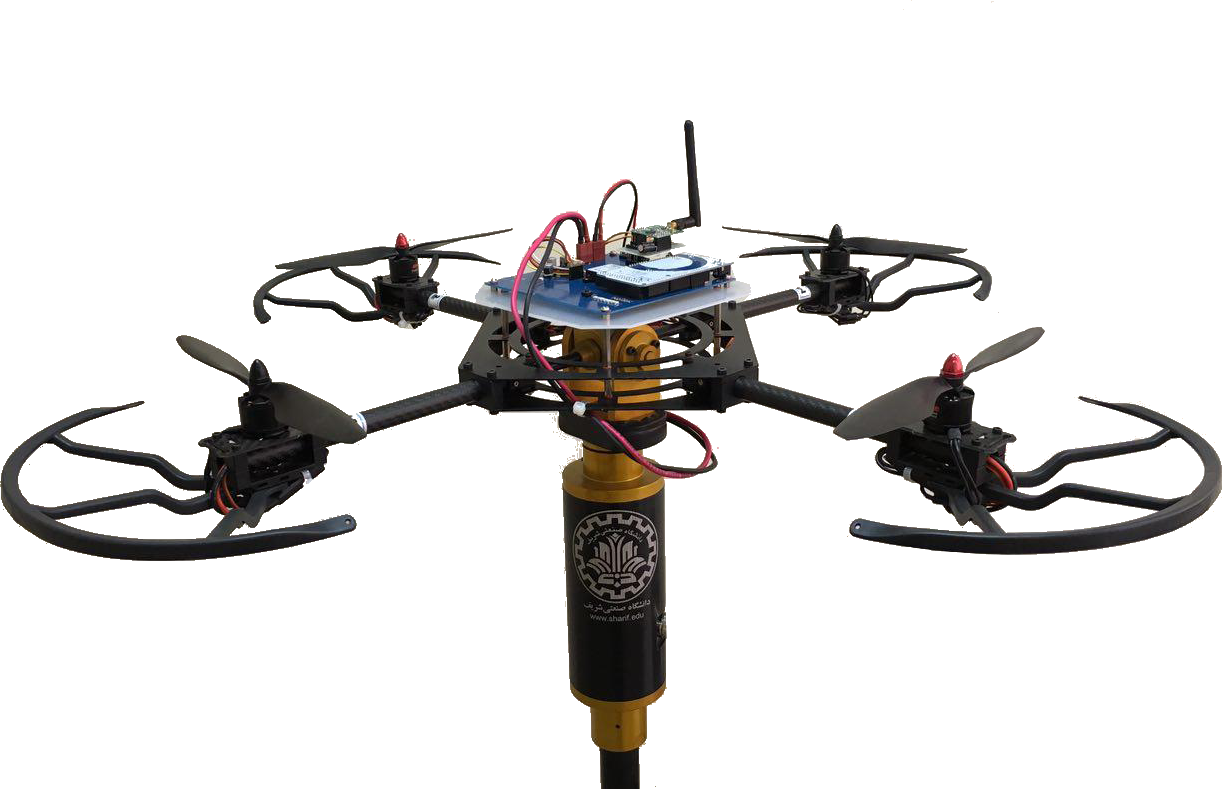
\includegraphics[width=0.5\textwidth]{../Figure/3DOFQuad.png}
  \caption{3-DoF Quadrotor platform.}
  \label{fig:quadrotor}
\end{figure}

\begin{figure}[H]
  \centering
  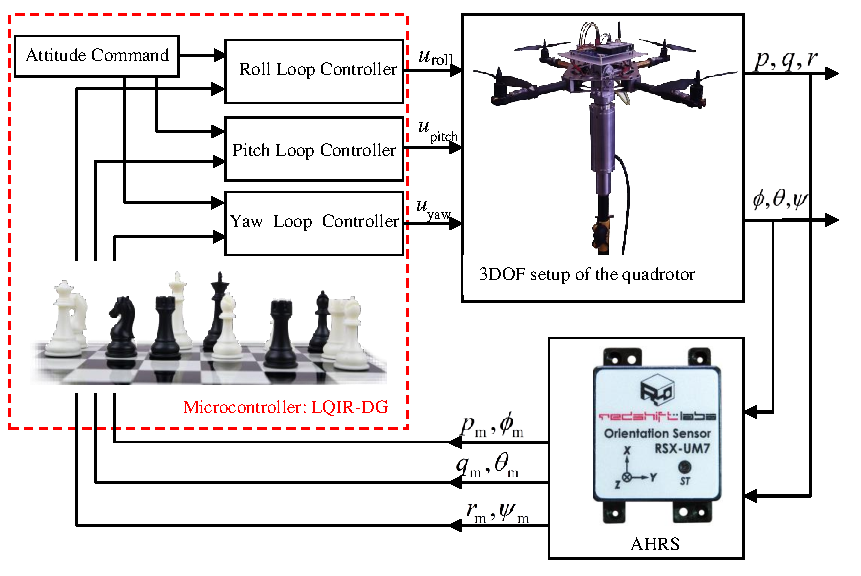
\includegraphics[width=0.5\textwidth]{../Figure/schematic.pdf}
  \caption{Graphical abstract of the LQIR-DG controller.}
  \label{fig:blockdiagram}
\end{figure}



% needed in second column of first page if using \IEEEpubid
%\IEEEpubidadjcol

\section{Model of the Quadrotor Platform}\label{sec:modeling}
Here, the quadrotor platform is modeled as nonlinear.
Then, a state-space model and a linear model are developed for control purposes to be utilized in the controller strategy.
Finally, a nonlinear identification method is applied to identify the parameters of the quadrotor.
\subsection{Quadrotor Configuration}
According to Figure \ref{fig:schematic}, the 3-DoF quadrotor schematic is including four rotors rotating the $z_B$ axis in the body frame with a rotational velocity, $\Omega_i~(i=1, 2, 3, 4)$. To eliminate the yawing moment, rotors (2, 4) and (1, 3) rotate clockwise and counter counterclockwise, respectively.

\begin{figure}[H]
  \centering
  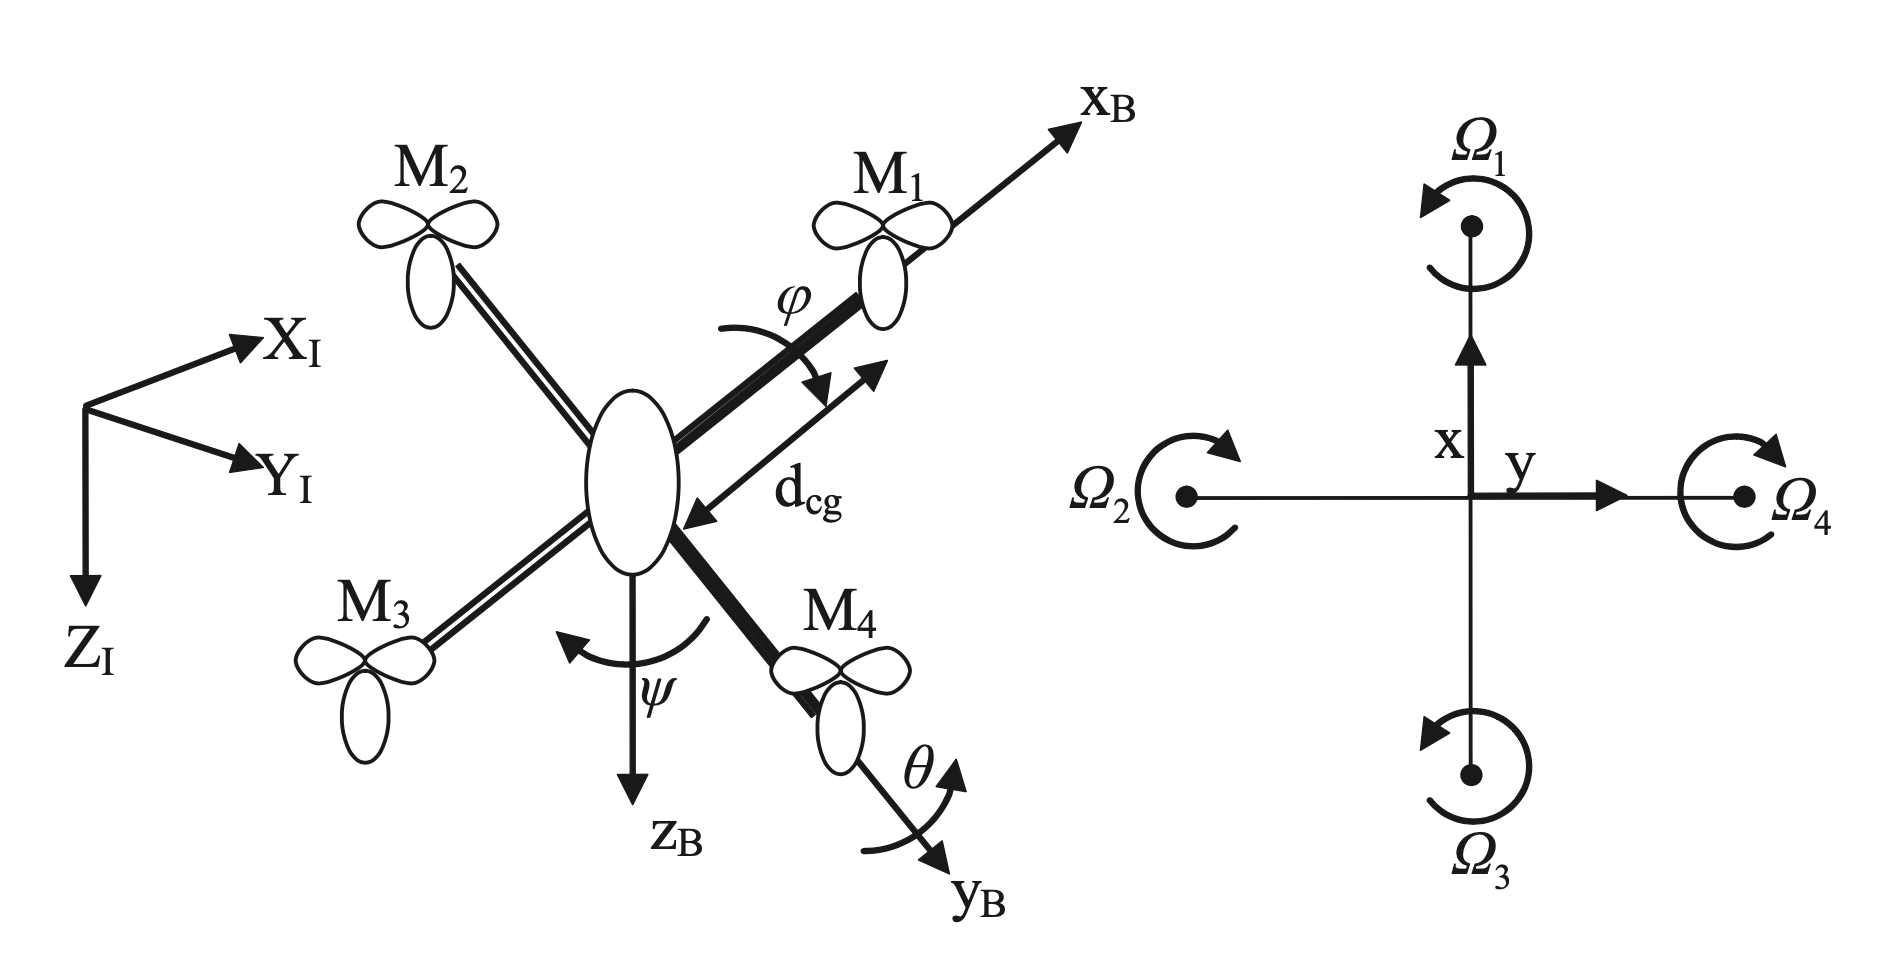
\includegraphics[width=0.5\textwidth]{../Figure/schematic.png}
  \caption{Quadrotor configuration.}
  \label{fig:schematic}
\end{figure}
\subsection{Dynamic Modeling of the Quadrotor Platform}
\noindent Here, according to Newton-Euler, the model of the quadrotor platform is presented as follows \cite{4399042, article_Bouabdallah}:
\begin{align}
  &\dot p = \dfrac{\mathrm{I}_{\text{yy}} - \mathrm{I}_{\text{zz}}}
  {\mathrm{I}_{\text{xx}}} qr + q \dfrac{\mathrm{I}_{\text{rotor}}}
  {\mathrm{I}_{\text{xx}}}\Omega_{c, r} + \dfrac{\mathrm{b\,d}_{\text{cg}} (\Omega_{c, 2}^2 - \Omega_{c, 4}^2)}{\mathrm{I}
  _{\text{xx}}} + \dfrac{d_{\text{roll}}}{\mathrm{I}_{\text{xx}}}
  \\
  &\dot q = \dfrac{\mathrm{I}_{\text{zz}} - 
  \mathrm{I}_{\text{xx}}}{\mathrm{I}_{\text{yy}}} rp +
  p \dfrac{\mathrm{I}_{\text{rotor}}}{\mathrm{I}_{\text{xx}}}\Omega_{c, r} + 
  \dfrac{\mathrm{b\,d}_{\text{cg}} (\Omega_{c, 1}^2 - \Omega_{c, 3}^2)}{\mathrm{I}_{\text{yy}}} +
  \dfrac{d_{\text{pitch}}}{\mathrm{I}_{\text{yy}}}
  \\
  &\dot r = \dfrac{\mathrm{I}_{\text{xx}} -
  \mathrm{I}_{\text{yy}}}{\mathrm{I}_{\text{zz}}} pq 
  +  \dfrac{\mathrm{d} (\Omega_{c, 1}^2 - \Omega_{c, 2}^2 + \Omega_{c, 3}^2 - \Omega_{c, 4}^2)}{\mathrm{I}_{\text{zz}}} 
  + \dfrac{d_{\text{yaw}}}{\mathrm{I}_{\text{zz}}}
  \end{align}
  where $\Omega_{c, i}~(i=1, 2, 3, 4)$ is the rotational velocity, computed as
  \begin{align}
      \Omega_{c, 1}^2 &= \Omega_{\text{mean}}^2 + \dfrac{1}{2\mathrm{b\,d}_{\text{cg}}}u_{\text{pitch}} + \dfrac{1}{4d}u_{\text{yaw}} \\
      \Omega_{c, 2}^2 &= \Omega_{\text{mean}}^2 + \dfrac{1}{2\mathrm{b\,d}_{\text{cg}}}u_{\text{roll}} - \dfrac{1}{4d}u_{\text{yaw}}\\
      \Omega_{c, 3}^2 &= \Omega_{\text{mean}}^2 - \dfrac{1}{2\mathrm{b\,d}_{\text{cg}}}u_{\text{pitch}} + \dfrac{1}{4d}u_{\text{yaw}} \\
      \Omega_{c, 4}^2 &= \Omega_{\text{mean}}^2 - \dfrac{1}{2\mathrm{b\,d}_{\text{cg}}}u_{\text{roll}} - \dfrac{1}{4d}u_{\text{yaw}}
  \end{align}
  In the above equation, $\Omega_{\text{mean}}$ is the rotational velocity of the rotors. Also, $\mathrm{d}_{\text{cg}}$, $\text{d}$, and $\text{b}$ represent the distance between the rotors and the gravity center, drag factor, and thrust factor, respectively.
$d_{\text{roll}}$, $d_{\text{pitch}}$, and $d_{\text{yaw}}$ denote the disturbances produced in the body coordinate frame. Additionally,
$u_{\text{roll}}$, $u_{\text{pitch}}$, and $u_{\text{yaw}}$ are control commands generated by the LQIR-DG controller. $\mathrm{I}_{\text{rotor}}$ is rotor inertia, and $\mathrm{I}_{\text{xx}}$, $\mathrm{I}_{\text{yy}}$, and $\mathrm{I}_{\text{zz}}$ are the moments of inertia.
Euler angle rates are also determined from angular body rates as follows:
\begin{equation}
	\begin{bmatrix}
	\dot\phi \\
	\dot\theta \\
	\dot\psi
	\end{bmatrix} = 
	\begin{bmatrix}
	1 & \sin(\phi)\tan(\theta) & \cos(\phi)\tan(\theta) \\
	0 & \cos(\phi) & -\sin(\phi) \\
	0 & \sin(\phi)/\cos(\theta) & \cos(\phi)/\cos(\theta)
	\end{bmatrix}
	\begin{bmatrix}
	p \\
	q \\
	r
	\end{bmatrix}
\end{equation}
The residual rotor velocity, denoted by $\Omega_{c,r}$, is calculated as follows:
\begin{equation}
	\Omega_{c, r} = -\Omega_{c, 1} + \Omega_{c, 2} - \Omega_{c, 3} + \Omega_{c, 4}
\end{equation}

\subsection{State-Space Formulation}\label{sec:state-space}
By defining $\boldsymbol{\mathrm{x}}_{\text{roll}} = \begin{bmatrix}
	x_1 & x_2
\end{bmatrix}^{\mathrm{T}}=
\begin{bmatrix}
	p & \phi
\end{bmatrix}^{\mathrm{T}}$
,
$\boldsymbol{\mathrm{x}}_{\text{pitch}} = \begin{bmatrix}
	x_3 & x_4 \end{bmatrix}^{\mathrm{T}} = 
	\begin{bmatrix}
	q & \theta \end{bmatrix}^{\mathrm{T}}
	$
	, and 
	$\boldsymbol{\mathrm{x}}_{\text{yaw}} = 
	\begin{bmatrix}
		x_5 & x_6
	\end{bmatrix}^{\mathrm{T}} = 
	\begin{bmatrix}
		r & \psi
	\end{bmatrix}^{\mathrm{T}}$, the formulation of the quadrotor platform is presented as follows:
\begin{align}\label{eq:diffeq}
	\dot x_1 &= \Gamma_1x_3 x_5 + \Gamma_2 x_3 \Omega_r + \Gamma_3\mathrm{b\,d}_{\text{cg}} (\Omega_{c, 1}^2 - \Omega_{c, 3}^2) + \Gamma_3d_{\text{roll}} \\[0.5em]
	\dot x_2 &= x_1 + (x_3\sin(x_2) + x_3\cos(x_2))\tan(x_4)
    \\[0.5em]
    \dot x_3 &= \Gamma_4 x_1 x_5 - \Gamma_5 x_1 \Omega_r +  \Gamma_6\mathrm{b\,d}_{\text{cg}} (\Omega_{c, 2}^2 - \Omega_{c, 4}^2) + \Gamma_6d_{\text{pitch}}\\[0.5em] \label{eq:diffeq-mid}
	\dot x_4 &= x_3\cos(x_4) - x_5\sin(x_2)\\[0.5em]
    \dot x_5 &= \Gamma_7x_1 x_3 +  \Gamma_8\mathrm{d} (\Omega_{c, 1}^2 - \Omega_{c, 2}^2 + \Omega_{c, 3}^2 - \Omega_{c, 4}^2) + \Gamma_8d_{\text{yaw}}\\[0.5em] 
    \dot x_6 &= (x_3\sin(x_4) + x_5\cos(x_2))/\cos(x_4) \label{eq:diffeq-end}
\end{align}
where $\Gamma_i (i = 1, \ldots, 8)$ is defined as
\begin{equation}
	\begin{split}
		\Gamma_1 &= \dfrac{\mathrm{I}_{\text{yy}} - \mathrm{I}_{\text{zz}}}{\mathrm{I}_{\text{xx}}}, \quad \Gamma_2 = \dfrac{\mathrm{I}_{\text{rotor}}}{\mathrm{I}_{\text{xx}}}, \quad \Gamma_3 = \dfrac{1}{\mathrm{I}_{\text{xx}}}\\ \Gamma_4 &= \dfrac{\mathrm{I}_{\text{zz}} - \mathrm{I}_{\text{xx}}}{\mathrm{I}_{\text{yy}}}, \quad \Gamma_5 = \dfrac{\mathrm{I}_{\text{rotor}}}{\mathrm{I}_{\text{xx}}}, \quad \Gamma_6 = \dfrac{1}{\mathrm{I}_{\text{yy}}} \\ \Gamma_7 &= \dfrac{\mathrm{I}_{\text{xx}} - \mathrm{I}_{\text{yy}}}{\mathrm{I}_{\text{zz}}}, \quad \Gamma_8 = \dfrac{1}{\mathrm{I}_{\text{zz}}}
	\end{split}
\end{equation}
The measurement vector, obtained from the AHRS, is presented as follows:
\begin{equation}
    \begin{split}
        \boldsymbol{\mathrm{z}} &= \begin{bmatrix}
        p \
        q \
        r \
        \phi \
        \theta \
        \psi
    \end{bmatrix}^\mathrm{T} + \boldsymbol{\nu}
    \end{split}
\end{equation}
where $\boldsymbol{\nu}$ is a Gaussian white noise. Moreover, the superscripts $\mathrm{T}$ indicate the transpose notation.
%%%? capital or small G g ? 
\subsection{Linear Model}
\noindent By defining $\boldsymbol{\dot{\mathrm{x}}} = \begin{bmatrix}
	\boldsymbol{{\mathrm{\dot x_{\text{roll}}}}}&
	\boldsymbol{{\mathrm{\dot x_{\text{pitch}}}}}&
	\boldsymbol{{\mathrm{\dot x_{\text{yaw}}}}}
\end{bmatrix}^{\mathrm{T}}$, the linear model of the quadrotor platform represented about the equilibrium points $(\boldsymbol{{\mathrm{x}}}_e^*\!=\!0$ and $\boldsymbol{{\mathrm{u}}}_e^*\!=\!0)$ as
\begin{equation}\label{eq:linear}
	\boldsymbol{\dot{\mathrm{x}}} = \boldsymbol{\mathrm{A\,x}} + 
	\boldsymbol{\mathrm{B}}
	\left(\boldsymbol{\mathrm{u}} + \boldsymbol{\mathrm{d}}\right)
\end{equation}
$\boldsymbol{\mathrm{A}}$ is the dynamic system matrix, denoted as
\begin{equation}
	\boldsymbol{\mathrm{A}} = \begin{bmatrix}
		\boldsymbol{{\mathrm{A_{\text{roll}}}}} & \boldsymbol{0} & \boldsymbol{0}\\
		\boldsymbol{0} & \boldsymbol{{\mathrm{A_{\text{pitch}}}}} & \boldsymbol{0} \\
		\boldsymbol{0} & \boldsymbol{0} & \boldsymbol{{\mathrm{A_{\text{yaw}}}}}
	\end{bmatrix}
\end{equation}
$
		\boldsymbol{\mathrm{A}}_{\text{roll}}  =\boldsymbol{\mathrm{A}}_{\text{pitch}}  = \boldsymbol{\mathrm{A}}_{\text{yaw}}  = \begin{bmatrix}
			0 & 0\\
			1 & 0
		\end{bmatrix}
$. Also, $\boldsymbol{\mathrm{B}}$ is the input matrix defined as
\begin{equation}
	\boldsymbol{\mathrm{B}} =
	\begin{bmatrix}
		\boldsymbol{{\mathrm{B_{\text{roll}}}}} & \boldsymbol{0} & \boldsymbol{0}\\
		\boldsymbol{0} & \boldsymbol{{\mathrm{B_{\text{pitch}}}}} & \boldsymbol{0} \\
		\boldsymbol{0} & \boldsymbol{0} & \boldsymbol{{\mathrm{B_{\text{yaw}}}}}
	\end{bmatrix}
\end{equation}
where $\boldsymbol{\mathrm{B}}_{\text{roll}}  = \begin{bmatrix}
	\dfrac{1}{\mathrm{I}_{\text{xx}}}
	&
	0
\end{bmatrix}^{\mathrm{T}}$, $\boldsymbol{\mathrm{B}}_{\text{pitch}}  = \begin{bmatrix}
	\dfrac{1}{\mathrm{I}_{\text{yy}}}
	&
	0
\end{bmatrix}^{\mathrm{T}}$, and $\boldsymbol{\mathrm{B}}_{\text{yaw}}  = \begin{bmatrix}
	\dfrac{1}{\mathrm{I}_{\text{zz}}}
	&
	0
\end{bmatrix}^{\mathrm{T}}$.
\subsection{Identification of the Platform Parameters}
\noindent In this section, the Nonlinear Least Squares (NLS) algorithm is utilized for estimating the model parameters ($\boldsymbol{\mathrm{\Gamma}}$) of the 3-DoF experimental platform using experimental data.
This technique is based on the Trust-Region Reflective (TRR) method, which finds the best values for $\boldsymbol{\mathrm{\Gamma}}$ by minimizing a cost function, defined as
\begin{equation}
	\min_{\Gamma}\left(\parallel e(\Gamma) \parallel^2\right) = 
	\min_{\Gamma} \left(\sum_{j=1}^{n}(\boldsymbol{z}_j- \tilde{\boldsymbol{z}}_j)(\boldsymbol{z}_j- \tilde{\boldsymbol{z}}_j)^\mathrm{T}\right)
\end{equation} %%%? what is j ??
where $\boldsymbol{z}$ and $\tilde{\boldsymbol{z}}$ are the experimental and simulated output signals when the same input signals are applied.
Moreover, $n$ is the number of scenarios.
To find a vector $\Gamma$, the optimization process performs until convergence is achieved. %%%?
The structure of the identification approach is illustrated in figure \ref{fig:identification}.
\begin{figure*}[h]
	\centering
    \resizebox{.8\textwidth}{!}{
	\begin{tikzpicture}[font=\small,thick]
		% Start block
		\node[draw, align=center,		minimum width=2.5cm,		minimum height=1cm, fill=blue!10] (block1) {\textbf{Experimental Data} \\Input: rotational velocity\\
		Output: attitude};
			
		% Voltage and Current Measurement
		\node[draw, align=center,		below=of block1,		minimum width=3.5cm,		minimum height=1cm, fill=blue!10	] (block2) {\textbf{Data Preprocessing} \\ Synchronization experimental, vs simulated data.};
		
		% Power and voltage variation
		
		\node[draw, align=center,		below=of block2,		minimum width=3.5cm,		minimum height=1cm, fill=blue!10	] (block3) {\textbf{NLS-TRR Optimization}\\
		Set bounds for parameters\\
		The set initial seed for all parameters\\
		Minimization of the cost function.};

		\node[draw, align=center,	below right=of block3,	minimum width=3cm,	minimum height=2.5cm,	fill=green!10	] (block_p) {{Identified parameters}\\
		$\boldsymbol\Gamma = \begin{bmatrix}\Gamma_1 &
			\Gamma_2 & \Gamma_3 & \Gamma_4\\
			\Gamma_5 & \Gamma_6 & \Gamma_7 & \Gamma_8
		\end{bmatrix}$};

		\node[draw, align=center,	below left=of block3,	minimum width=3cm,	minimum height=2.5cm,	fill=red!10	] (block_s) {{simulated model}\\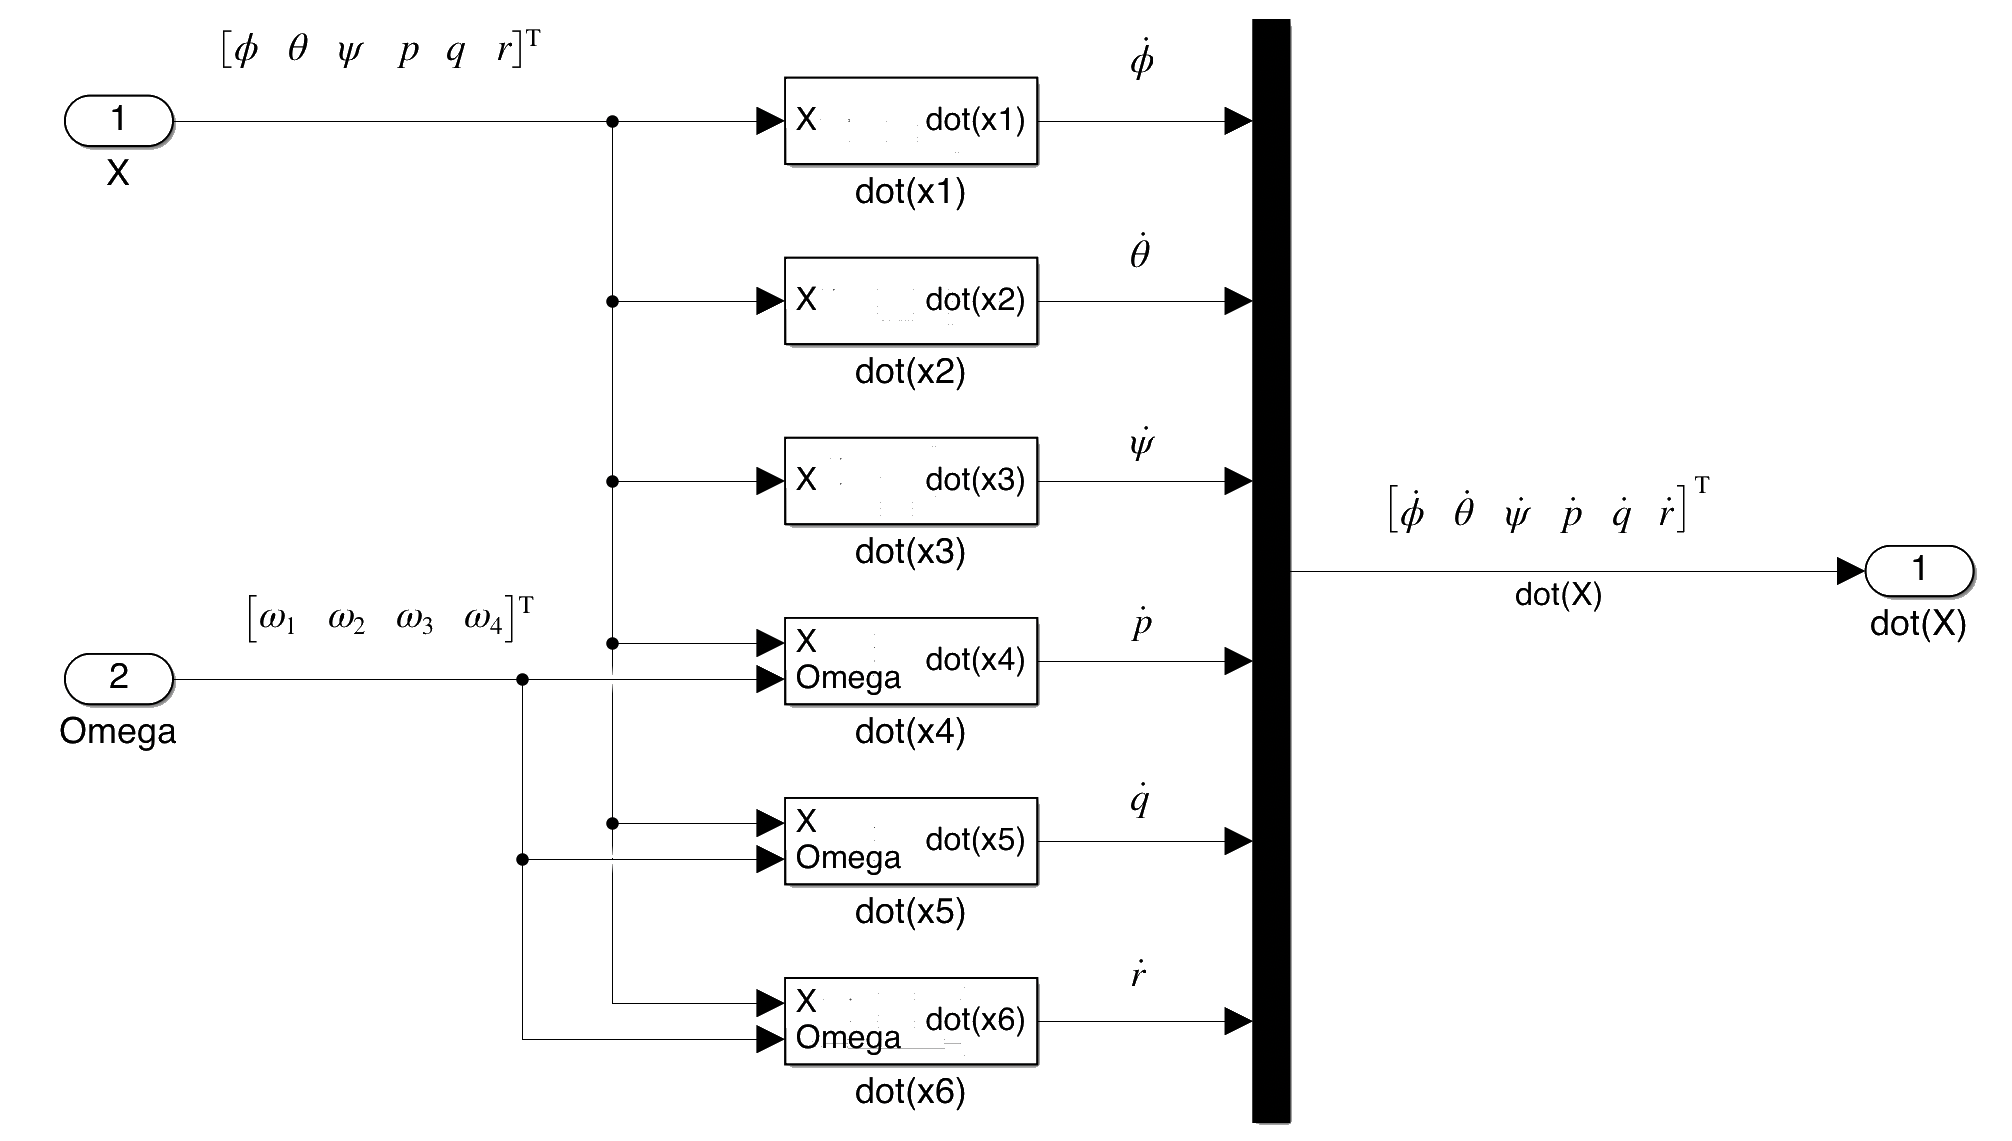
\includegraphics[scale=.05]{../Figure/All-six.png}};
		
		% Conditions test
		\node[draw,		diamond,		below =4cm of block3,		minimum width=2.5cm,		inner sep=0,		fill=yellow!10	] (block4) { Error $< \delta$};
		
		\node[draw,		below=1.5cm of block4,		minimum height=1cm,		minimum width=2.5cm,		inner sep=0,		fill=blue!10	] (block5) {End};
		
		\node[draw,		right=2cm of block4,		minimum height=1cm,		minimum width=2.5cm,		fill=red!10		] (block6) {Insufficient experimental data};
				
		 
		 
		% Arrows
		\draw[-latex] (block1) edge (block2)
			(block2) edge (block3)
			(block3) -| (block_s);
			% (block3) edge (block_p);
	
		\draw[-latex] (block3) -| (block_p);
	
		\draw[-latex] (block_s) -| (block4);
	
		\draw[-latex] (block_p) -| (block4);
	
		\draw[stealth-stealth] (block_s) -- (block_p);
		 
		\draw[-latex] (block4) -- (block5)
			node[pos=0.5,fill=white,inner sep=0]{Yes};
		 
		\draw[-latex] (block4) -- (block6)
			node[pos=0.5,fill=white,inner sep=0]{No};
	
		\coordinate[left=5.5cm of block3] (aux);
		\coordinate[right= of block_p] (aux1);
		% \draw[-latex] (block6) |- (block2);
		\draw[-latex] (block1) -| (aux) |- (block4);
		\draw[-latex] (block6) -| (aux1) |- (block1);
		\end{tikzpicture}
        }
		\caption{Structure of TRRLS identification approach.}
		\label{fig:identification}
\end{figure*}

\section{LQIR-DG Controller Structure}\label{sec:controller}
\noindent First, the augmented states of the quadrotor platform, including the states and their integrals are selected to use in the structure of the LQIR-DG controller for eliminating the steady-state errors. Then, the design methodology of the controller structure is introduced to produce the best commands for the 3-DoF quadrotor platform.
\subsection{Augmented States}
\noindent To augment an integral action into the control strategy architecture, the augmented states are defined as $\boldsymbol{\mathrm{x_{a}}} = \begin{bmatrix}
	\boldsymbol{\mathrm{x}} &
	\displaystyle\int\boldsymbol{\mathrm{x}}
\end{bmatrix}^\mathrm{T}$. Then, the quadrotor platform model, utilized in the controller structure, is presented as

\begin{equation}\label{systemlqidg}
	\begin{split}
		\boldsymbol{\dot{\mathrm{x}}_a} &= \begin{bmatrix}
			\boldsymbol{\mathrm{A}} & \boldsymbol{0}\\
			\boldsymbol{\mathrm{I}} & \boldsymbol{0}
		\end{bmatrix}\boldsymbol{\mathrm{x_a}} + \begin{bmatrix}
			\boldsymbol{\mathrm{B}}\\
			\boldsymbol{0}
		\end{bmatrix}
		 \left(\boldsymbol{\mathrm{u}} + \boldsymbol{\mathrm{d}}\right)%, \quad \boldsymbol{x}(0) = 
	\end{split}
\end{equation}
The notation $\boldsymbol{\mathrm{I}}$ denotes the identity matrix.
\subsection{LQIR-DG Control Scheme with Integral Action}
\noindent In the proposed controller scheme, two fundamental players are selected in accordance with the game theory approach. The primary player determines the control commands, while another player generates the worst possible disturbance.
To achieve the primary objective, the first player minimizes the following cost function but the other player maximizes it:
\begin{equation}\label{eq:min_max_cost_function}
	\begin{split}
		&\min_{u} \max_{d} J(\boldsymbol{\mathrm{x_{a_i}}}, {d_i}, {u_i})= \\ 
		&\min_{d} \max_{u}
		\int_{0}^{\mathrm{t_f}}\biggl (\boldsymbol{\mathrm{x^\mathrm{T}_{a_i}}}  \boldsymbol{\mathrm{Q_i}} \boldsymbol{\mathrm{x_{a_i}}}+
	   {{u^\mathrm{T}_i}}  {{R}} {{u_i}}-
	   {{d^\mathrm{T}_{i}}} {{ R_{d} d_{i}}}
	   \biggl )\mathrm{d}t
	\end{split}
\end{equation}
where $\mathrm{t_f}$ is the stop time and $i$-index denotes the roll, pitch, and yaw channels of the quadrotor. $\boldsymbol{\mathrm{Q_i}}$, ${{R_{d}}}$, and ${{R}}$ are weight coefficients of the cost function.
By solving the above problem, the optimal control command is computed as follows \cite{LQDG}:
\begin{equation}
	{{u_i}} = -\boldsymbol{{\mathrm{K}}_{i}} \boldsymbol{{\mathrm{x_{a_i}}}}
\end{equation}
Moreover, the worst disturbance is obtained as
\begin{equation}
	{{d_i}} =\boldsymbol{{\mathrm{K_{d_i}}}}\boldsymbol{{\mathrm{x_{a_i}}}}
\end{equation}
Here, $\boldsymbol{{\mathrm{K_{d_i}}}}$ and $\boldsymbol{{\mathrm{K_i}}}$ are gain values defined as follows:
\begin{align}
	\boldsymbol{{\mathrm{K_{d_i}}}} &= {{{R}}^{-1}_{d}}\boldsymbol{{\mathrm{B}_{a_{d_i}}^\mathrm{T}}}\boldsymbol{{\mathrm{P}}_{a_{d_i}}}\\
	\boldsymbol{{\mathrm{K_i}}} &= {{{R}}^{-1}}\boldsymbol{{\mathrm{B}_{a_i}^\mathrm{T}}}\boldsymbol{{\mathrm{P}}_{a_i}}
\end{align}
$\boldsymbol{{\mathrm{P}}_{a_i}}$ and $\boldsymbol{{\mathrm{P}}_{a_{d_i}}}$ satisfy
\begin{align}\label{coupled_riccatti_LQIDG}
	&-\boldsymbol{\mathrm{A^\mathrm{T}_a}}\boldsymbol{\mathrm{P_{a_{d_i}}}}
	 - \boldsymbol{\mathrm{Q_{i}}} - \boldsymbol{\mathrm{P_{a_{d_i}}}}\boldsymbol{\mathrm{A_a}} 
	 + \boldsymbol{\mathrm{P_{a_{d_i}}}}\boldsymbol{\mathrm{S_{a_i}}}\boldsymbol{\mathrm{P_{a_i}}}
	  +\boldsymbol{\mathrm{P_{a_{d_i}}}}\boldsymbol{\mathrm{S_{a_{d_i}}}}\boldsymbol{\mathrm{P_{a_{d_i}}}}
	=\boldsymbol{\mathrm{0}}\\
            &-\boldsymbol{\mathrm{A^\mathrm{T}_a}}\boldsymbol{\mathrm{P_{a_i}}} - \boldsymbol{\mathrm{Q_i}}
			 - \boldsymbol{\mathrm{P_{a_i}}}\boldsymbol{\mathrm{A_a}}  +
			  \boldsymbol{\mathrm{P_{a_i}}}\boldsymbol{\mathrm{S_{a_{d_i}}}}\boldsymbol{\mathrm{P_{a_{d_i}}}} 
			  +\boldsymbol{\mathrm{P_{a_i}}}\boldsymbol{\mathrm{S_{a_i}}}\boldsymbol{\mathrm{P_{a_i}}} =\boldsymbol{\mathrm{0}}
\end{align}
where $
	\boldsymbol{\mathrm{S_{a_i}}} = \boldsymbol{\mathrm{B_{a_i}}}R^{-1}\boldsymbol{\mathrm{B}^\mathrm{T}_{a_i}}$ and $
	\boldsymbol{\mathrm{S{a_{d_i}}}} = \boldsymbol{\mathrm{B}_{a_{d_i}}}R_{d}^{-1}\boldsymbol{\mathrm{B}^\mathrm{T}_{a_{d_i}}}.
$%%%? needd : or not


\section{Results}\label{sec:results}
\noindent The results of the parameter identification and the LQIR-DG Controller for the quadrotor platform are presented. First, the quadrotor parameters are estimated based on the NLS method. Then, performance of the LQIR-DG structure is evaluated.
Tables \ref{tab:parameters} and \ref{tab:control weight_new} present the quadrotor and LQIR-DG parameters, respectively.
\begin{table*}[h]
	\centering
	\caption{Quadrotor parameters}
	\renewcommand{\arraystretch}{1.3}
	\begin{center}
	\begin{tabular}{c c c c c c}
	\hline
	Parameter & Unit & Value & Parameter & Unit & Value \\
	\hline
	$\mathrm{d}_{\text{cg}}$ & $\mathrm{m}$ & $0.2$ & $\mathrm{I}_{\text{xx}}$ & $\mathrm{kg.m^2}$ & $0.02839$ \\ 
	$\mathrm{d}$ & $\mathrm{N.m.\sec^2/rad^2}$ & $3.2\times10^{-6}$ &
	$\mathrm{I}_{\text{yy}}$ & $\mathrm{kg.m^2}$ & $0.03066$ \\
	$\mathrm{b}$ & $\mathrm{N.\sec^2/rad^2}$ & $3.13\times10^{-5}$ 
	& $\mathrm{I}_{\text{zz}}$ & $\mathrm{kg.m^2}$ & $0.0439$ \\
	$\Omega_{\text{mean}}$ & $\mathrm{rpm}$ & $2000$ & $\mathrm{I}_{\text{rotor}}$ & $\mathrm{kg.m^2}$ & $4.4398\times 10^{-5}$ \\
	\hline
\end{tabular}
\label{tab:parameters}
\end{center}
\end{table*}
\begin{table}[H]
	\centering
	\caption{LQIR-DG controller parameters}
	\renewcommand{\arraystretch}{1.3}
	\begin{tabular}{@{}ccc@{}}
	\toprule
	Channel & Weighting Matrix & Values \\
	\midrule
	Roll & $\mathbf{Q_{roll}}$ & $\text{diag}([0.02, 65.96, 83.04, 0.00])$ \\
	Pitch & $\mathbf{Q_{pitch}}$ & $\text{diag}([435.01, 262.60, 262.60, 0.00])$ \\
	Yaw & $\mathbf{Q_{yaw}}$ & $\text{diag}([4 \times 10^{-4}, 0.00, 0.133, 0])$ \\
	-& $R$ & $1$ \\
	-&$R_d$ & $1.2764$ \\
	\bottomrule
	\end{tabular}
	\label{tab:control weight_new} %%%? R in above is not matrix i have changed
	%%%? need to know where weighting matrix came from
\end{table}
\subsection{Identification of the 3-DoF quadrotor platform model}
\noindent As described in section \ref{sec:state-space}, the parameters of the quadrotor platform, denoted by $\Gamma_i (i=1, ..., 8)$, are identified using the NLS-TRR algorithm.
To increase the accuracy of parameter identification, three scenarios are considered according to Table \ref{tab:identification}.
In the first scenario, depicted in Figure \ref{fig:one_degree_identification}, the quadrotor rotates about only one axis (roll, pitch, or yaw axes) to identify the parameters $\Gamma_3$, $\Gamma_6$, and $\Gamma_8$.
In the second scenario, according to Figure \ref{fig:two_degree_identification}, the parameters $\Gamma_2$ and $\Gamma_5$ are estimated by rotating the experimental platform around its roll and pitch axes simultaneously. Finally, Figure \ref{fig:three_degree_identification} displays the results of the third scenario including the estimation of the parameters $\Gamma_1$, $\Gamma_4$, and $\Gamma_7$ for the UAV model, when the platform freely rotates around three axes.
After the termination condition is met, the optimal values of the quadrotor parameters are computed and denoted in Table \ref{tab:true_parameters}. 
These results illustrate that the outputs of the simulation results for the quadrotor model are consistent with reality.
\begin{table*}[h]
	\caption{Scenarios for identification of quadrotor parameters.}
	\centering
	\begin{adjustbox}{max width=\textwidth}
	\begin{tabular}{c c *{3}{wc{\myleneiler}} *{4}{wc{\mylenomega}}}
	\toprule
	\multirow{2}{*}{Scenario} & \multirow{2}{*}{Description}
	& \multicolumn{3}{c}{Initial Condition (deg)} &
	\multicolumn{4}{c}{Rotational Velocity Commands (rpm)} \\
	\cmidrule(lr){3-5} \cmidrule(lr){6-9}
	& & $\phi_0$ & $\theta_0$ & $\psi_0$ & $\Omega_1$ & $\Omega_2$ & $\Omega_3$ & $\Omega_4$\\
	\midrule
	\multirow{3}{*}{I} & roll free & 38 & - & - & 2000 & 2000 & 2000 & 3400\\
	& pitch free & - & -15 & - & 3700 & 2000 & 2000 & 2000 \\
	& yaw free & -& - &-75 & 2000 & 3300 & 2000 & 3300 \\
	\midrule
	II & roll \& pitch free &8 & -5 & - & 1700 & 3800 & 2400 & 1700\\
	\midrule
	III & roll, pitch, \& yaw free &
	8 & -3 & -146 & 1700 & 3800 & 2400 & 1700 \\
	\bottomrule
	\end{tabular}
	\end{adjustbox}
	\label{tab:identification}
\end{table*}


\begin{table}[H]
	\renewcommand{\arraystretch}{1.3}
	\caption{True values of the quadrotor parameters.}
	\begin{center}
	\begin{tabular}{c c c c}
	\hline
	Parameter & Value & Parameter & Value  \\
	\hline
	$\Gamma_1$ & $-0.9622$ & $\Gamma_5$ & $3.6441\times10^{-4}$ \\

	$\Gamma_2$ & $-0.0154$ & $\Gamma_6$ & $7.5395\times10^{-5}$ \\

	$\Gamma_3$ &$5.4716\times10^{-5}$ & $\Gamma_7$ & $0.1308$ \\

	$\Gamma_4$ & $1.0457$ & $\Gamma_8$ & $4.3753\times10^{-5}$ \\
	\hline
	\end{tabular}
	\label{tab:true_parameters}
	\end{center}
\end{table}
\begin{figure}[H]
	\centering
	\subfloat[]{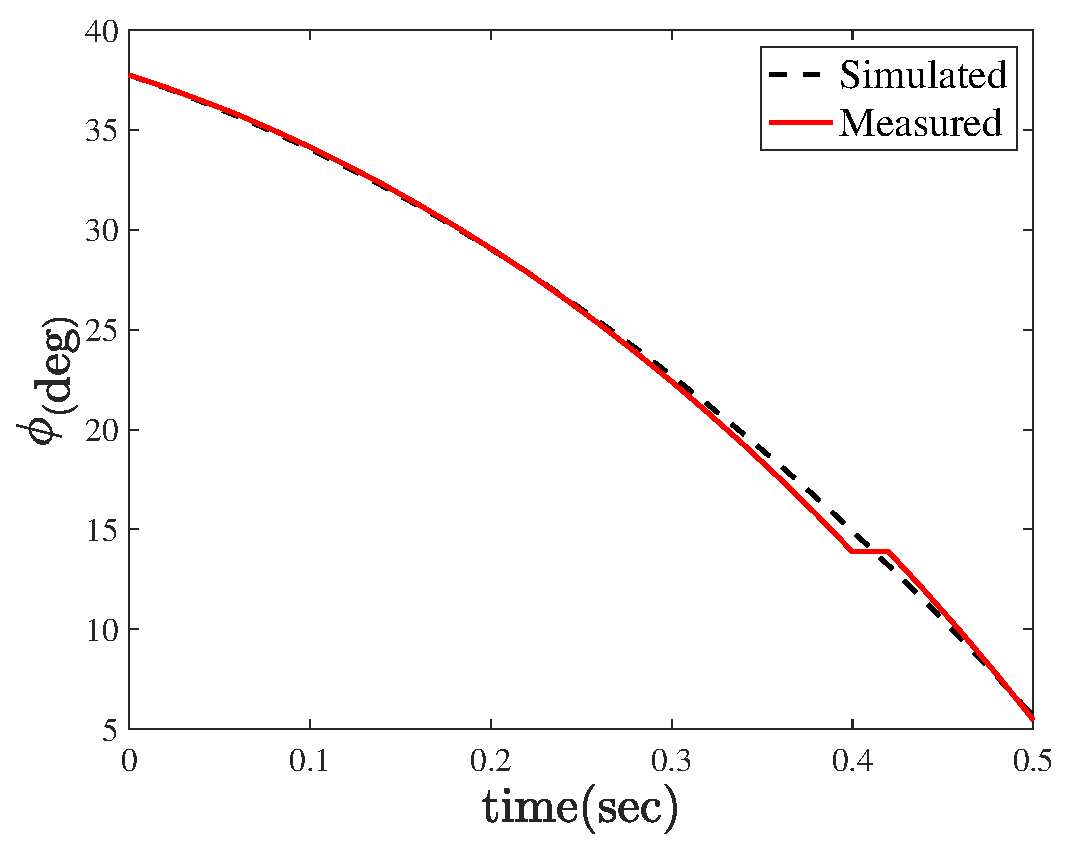
\includegraphics[width=.5\linewidth]{../Figure/parameter_estimation/roll/roll}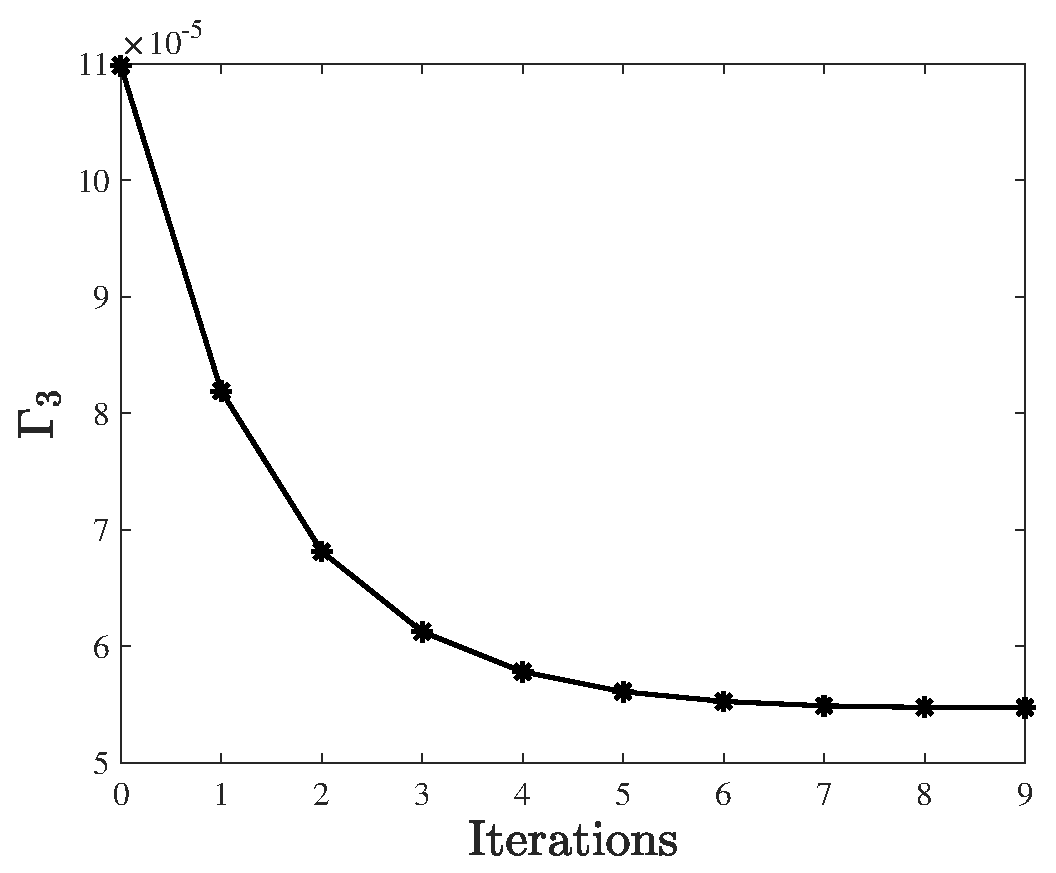
\includegraphics[width=.5\linewidth]{../Figure/parameter_estimation/roll/roll_parameter}
	}
	\hfil
	% \vspace{-0.25cm}
	\subfloat[]{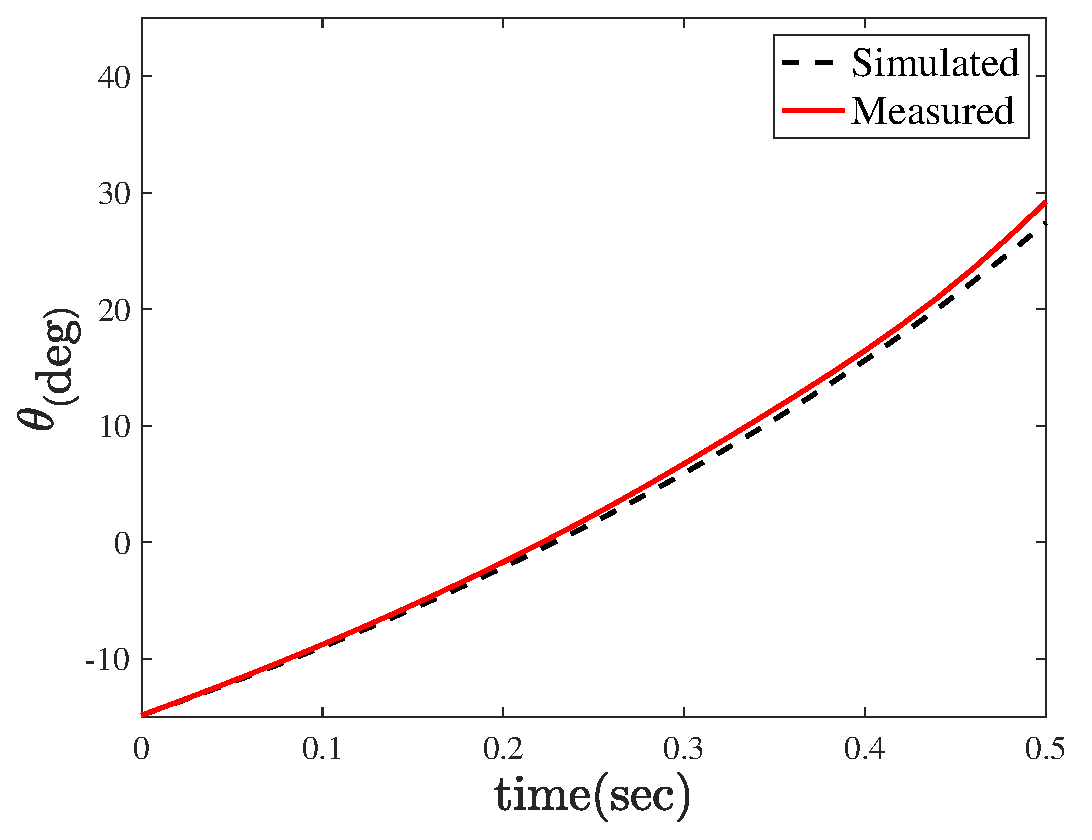
\includegraphics[width=.5\linewidth]{../Figure/parameter_estimation/pitch/pitch}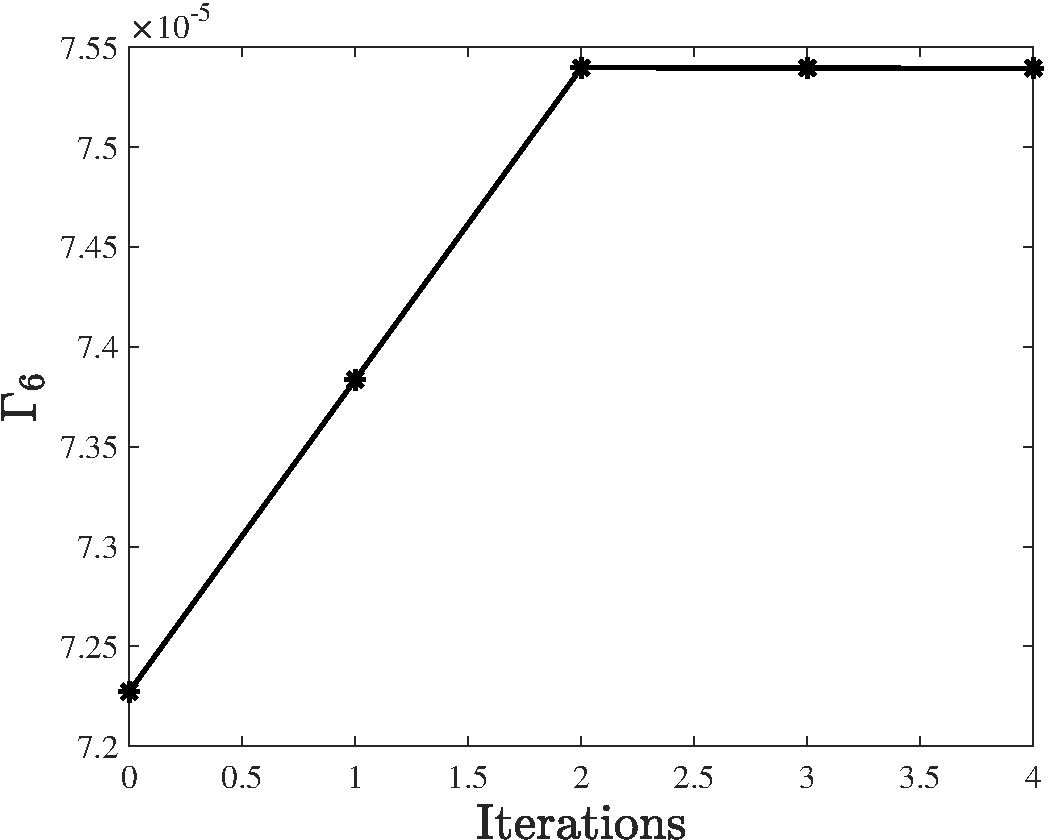
\includegraphics[width=.5\linewidth]{../Figure/parameter_estimation/pitch/pitch_parameter}
	}
	\hfil
	% \vspace{-0.25cm}
	\subfloat[]{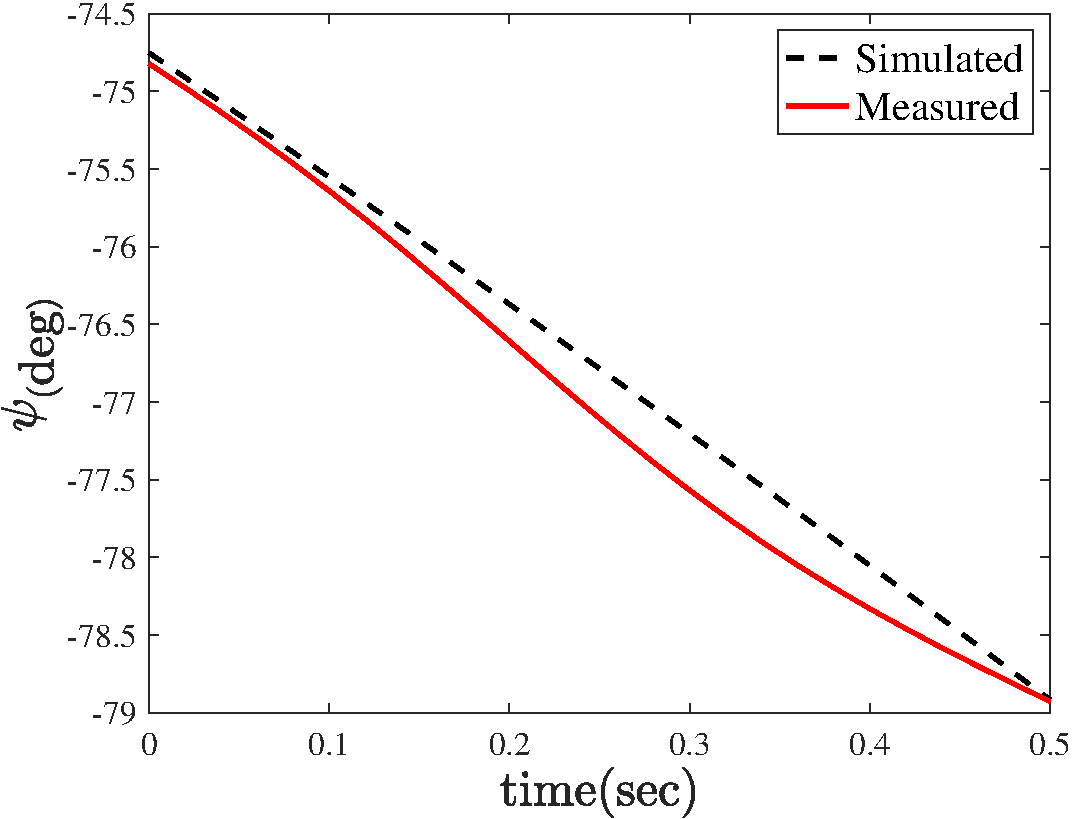
\includegraphics[width=.5\linewidth]{../Figure/parameter_estimation/yaw/yaw}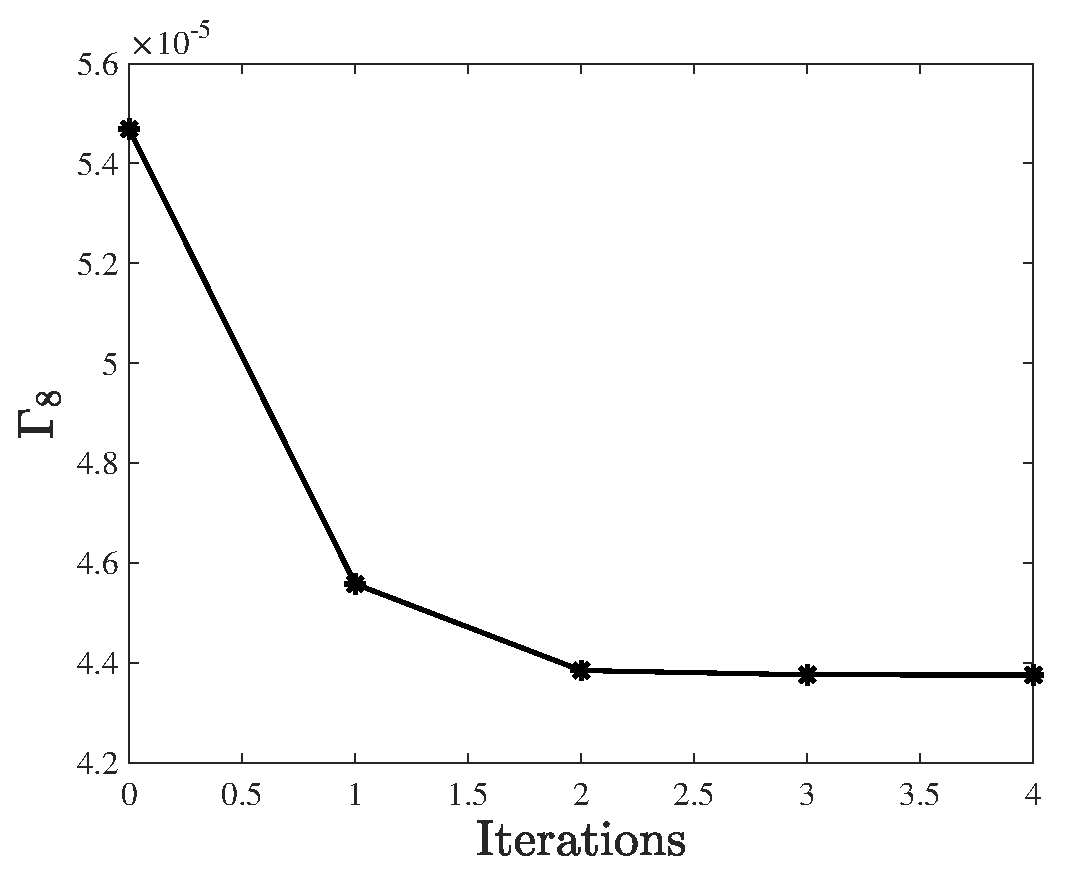
\includegraphics[width=.5\linewidth]{../Figure/parameter_estimation/yaw/yaw_parameter}
	}
	\caption{Identification process results when the quadrotor rotates about only one axis: (a) identification of $\Gamma_3$ in free roll motion. (b) identification of $\Gamma_6$ in free pitch motion. (c) identification of $\Gamma_8$
	in free yaw motion.}
	\label{fig:one_degree_identification}
\end{figure}
\begin{figure}[H]
	\centering
	\subfloat[]{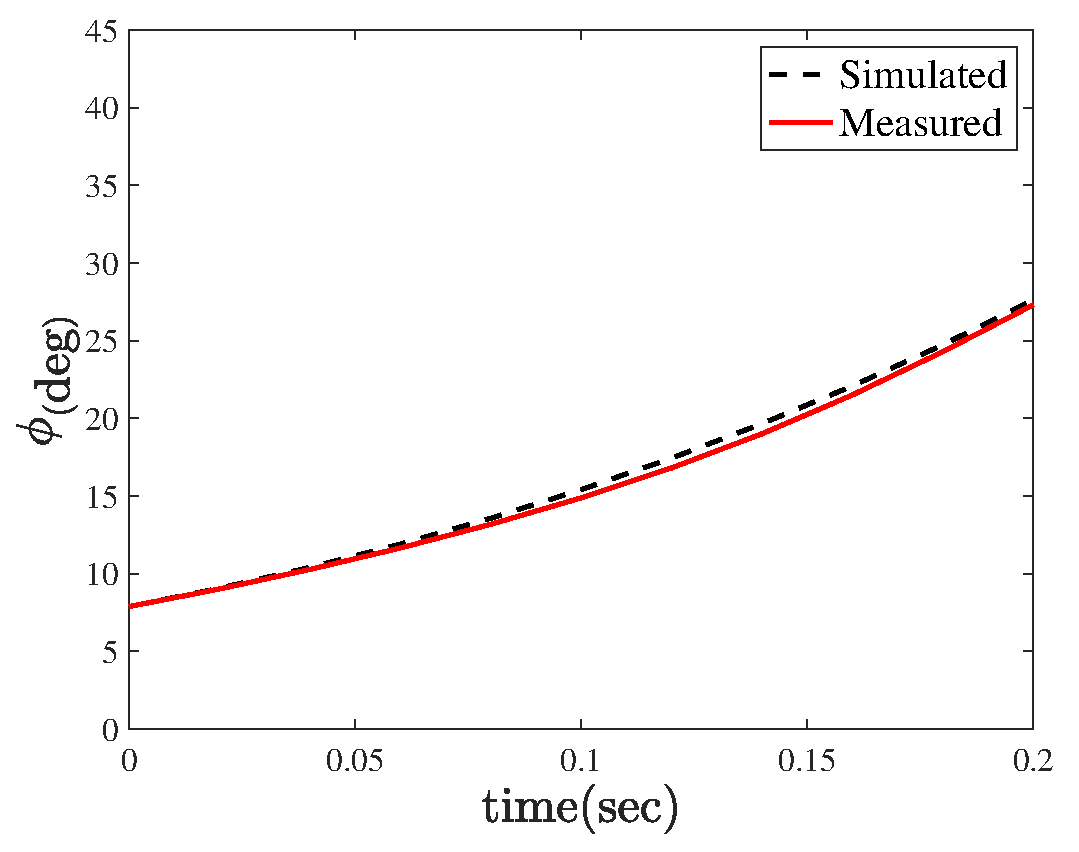
\includegraphics[width=.5\linewidth]{../Figure/parameter_estimation/roll-pitch/roll}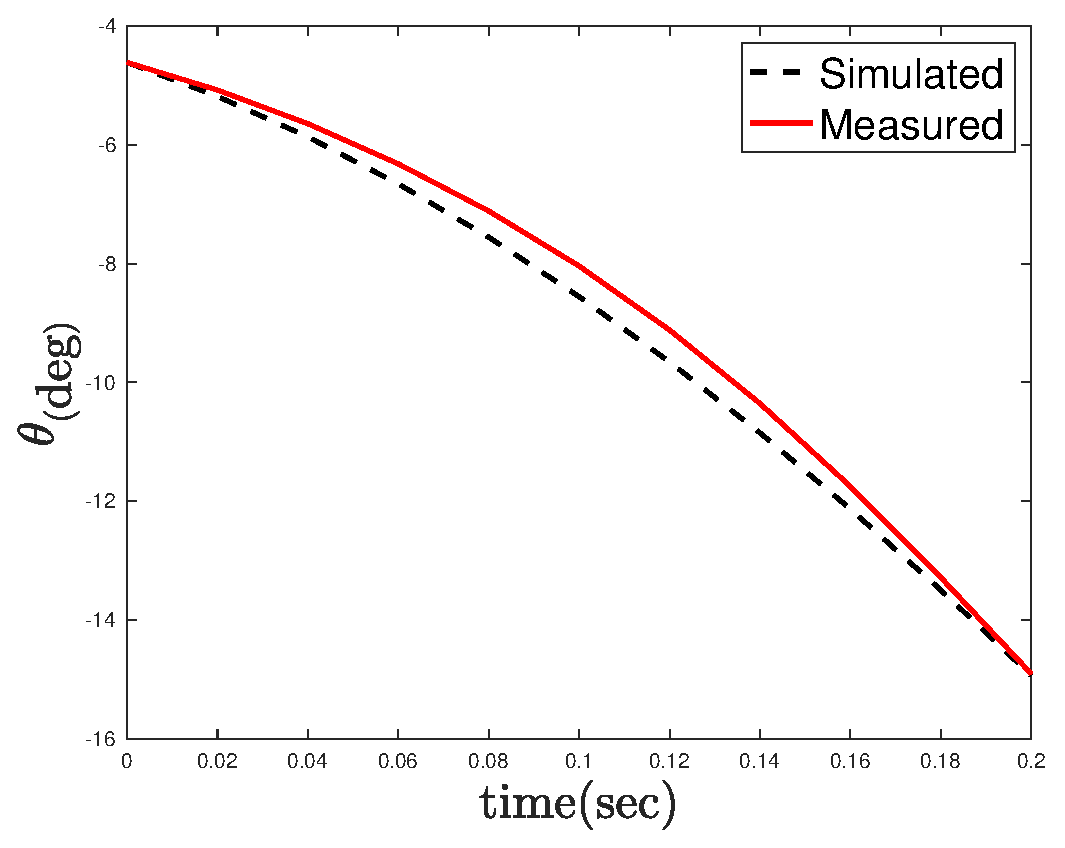
\includegraphics[width=.5\linewidth]{../Figure/parameter_estimation/roll-pitch/pitch}
	}
	\hfil
	% \vspace{-0.25cm}
	\subfloat[]{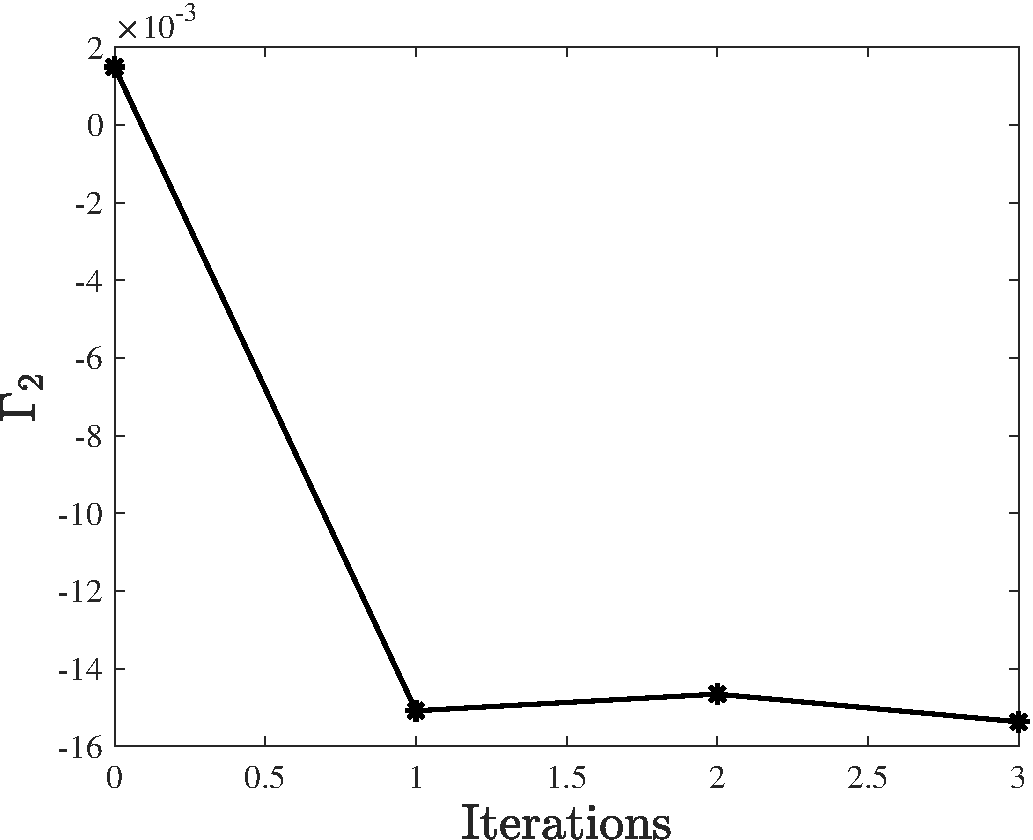
\includegraphics[width=.5\linewidth]{../Figure/parameter_estimation/roll-pitch/roll_parameter}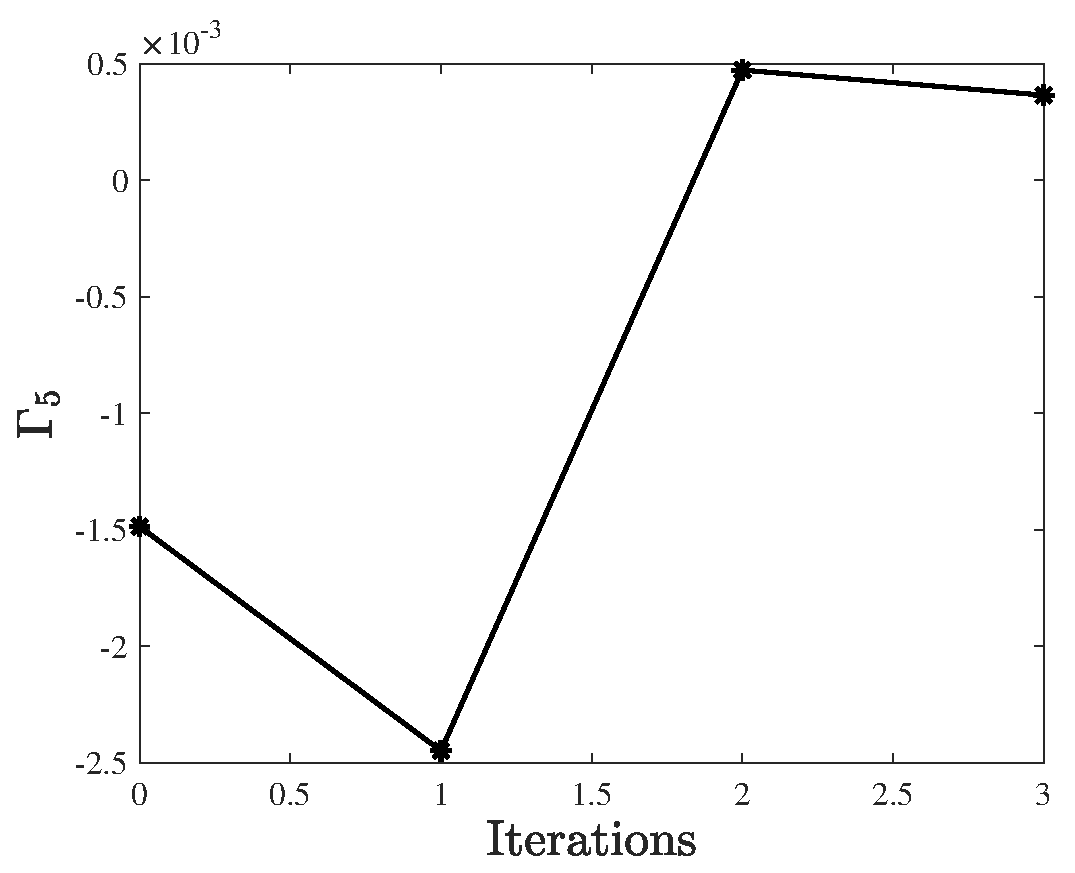
\includegraphics[width=.5\linewidth]{../Figure/parameter_estimation/roll-pitch/pitch_parameter}
	}
	\caption{Identification process results when the quadrotor rotates about its roll and pitch axes:
	(a) comparison of simulation and experimental results. (b) identification of $\Gamma_2$ and $\Gamma_5$.}
	\label{fig:two_degree_identification}
\end{figure}
\begin{figure}[H]
	\centering
	\subfloat[]{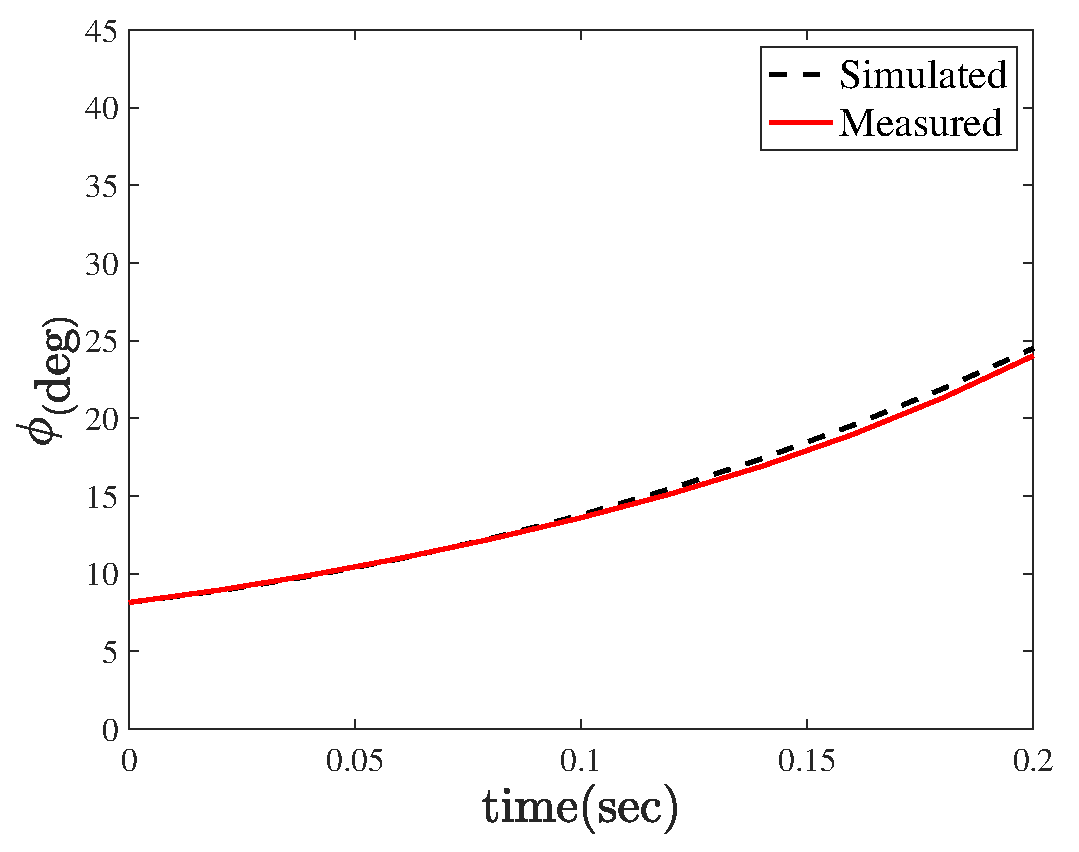
\includegraphics[width=.33\linewidth]{../Figure/parameter_estimation/3DOF/roll}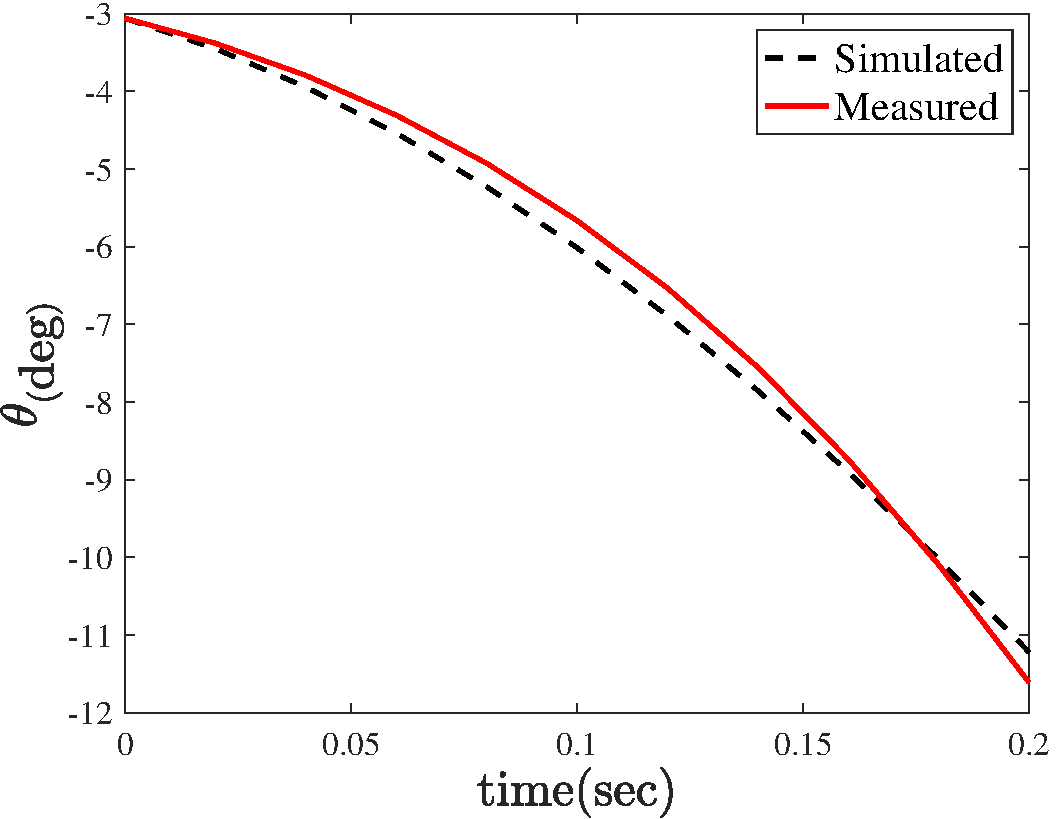
\includegraphics[width=.33\linewidth]{../Figure/parameter_estimation/3DOF/pitch}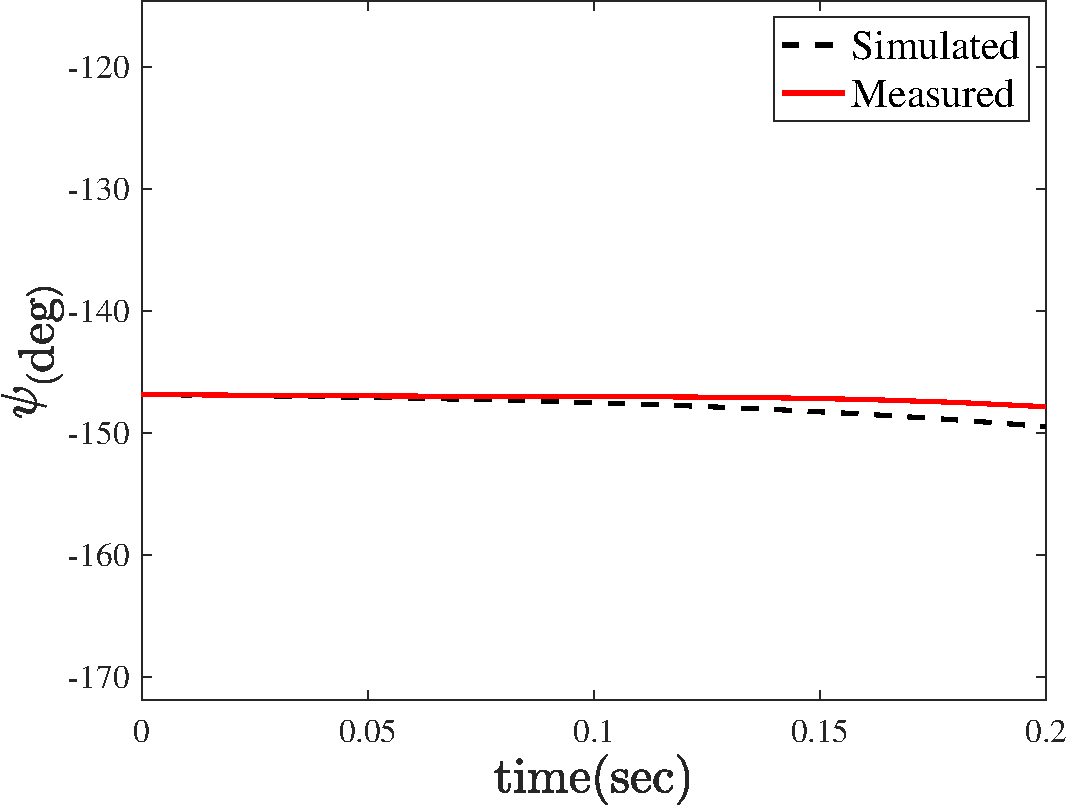
\includegraphics[width=.33\linewidth]{../Figure/parameter_estimation/3DOF/yaw}
	}
	\hfil
	\subfloat[]{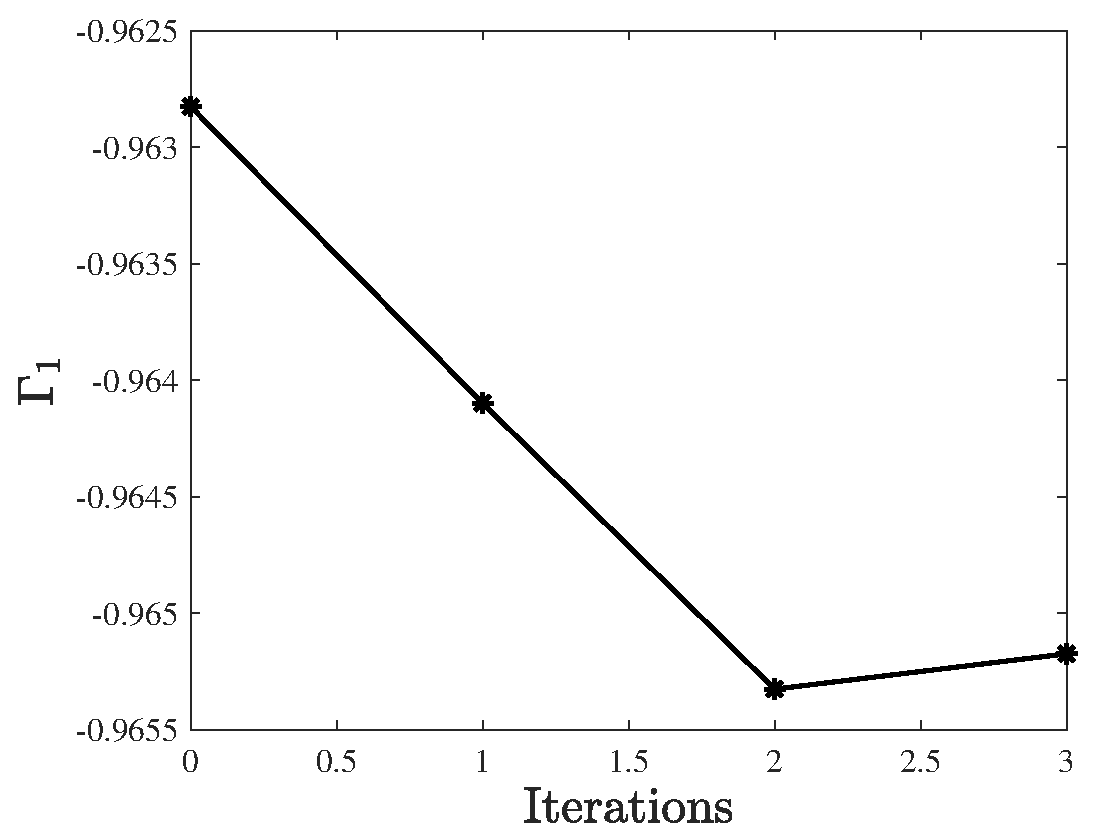
\includegraphics[width=.33\linewidth]{../Figure/parameter_estimation/3DOF/roll_parameter}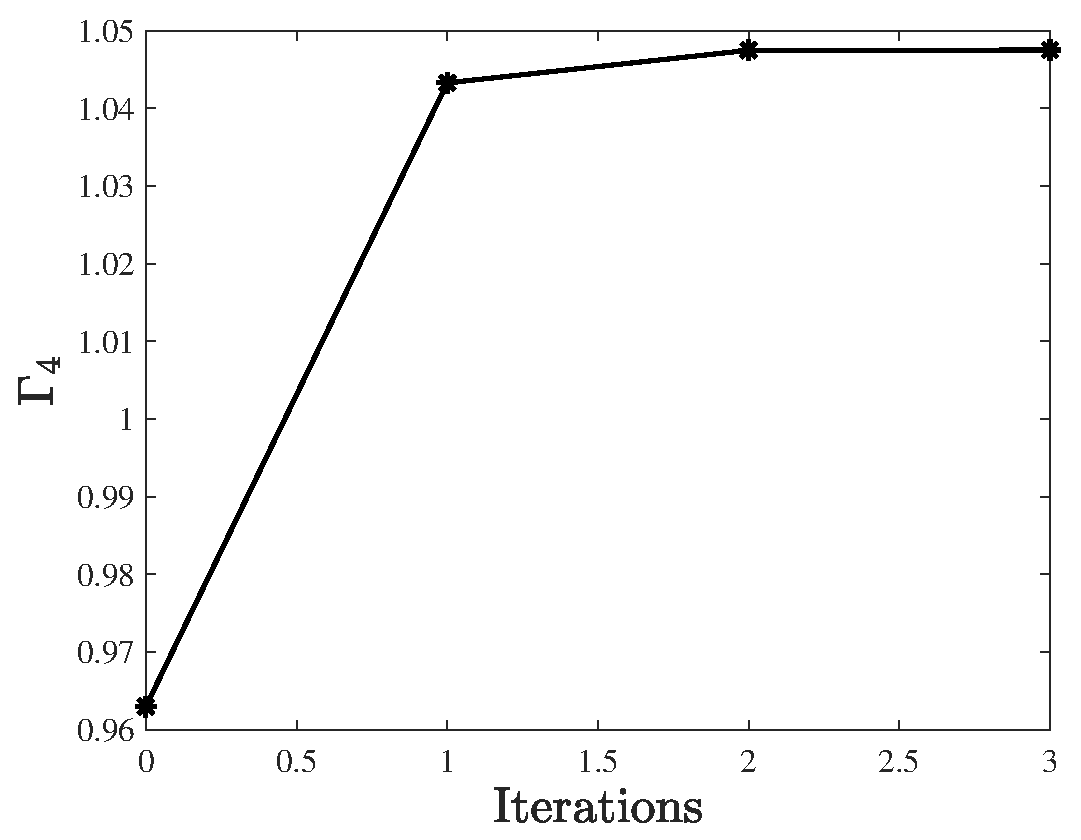
\includegraphics[width=.33\linewidth]{../Figure/parameter_estimation/3DOF/pitch_parameter}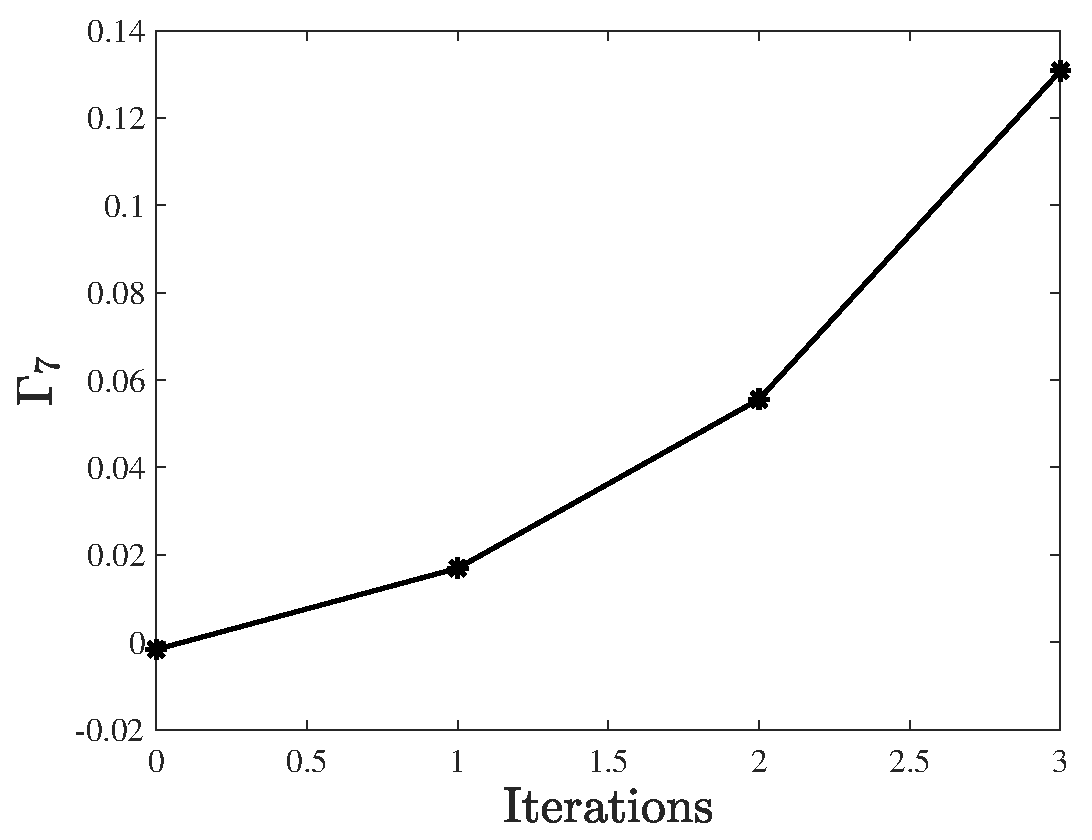
\includegraphics[width=.33\linewidth]{../Figure/parameter_estimation/3DOF/yaw_parameter}
	}
	\caption{Identification process results when the quadrotor rotates about its roll, pitch, and yaw axes: (a) comparison of simulation and experimental results. (b) identification of $\Gamma_1$ , $\Gamma_4$ and
	$\Gamma_7$ parameters.}
	\label{fig:three_degree_identification}
\end{figure}
\subsection{Evaluation of LQIR-DG Performance}
\noindent In this section, the LQIR-DG controller algorithm is evaluated in three scenarios i) regulation and tracking problems, ii) disturbance rejection, and iii) impact of model uncertainty.
Finally, a comparison of the proposed controller is performed with a PID controller and variants of the LQR controller. 
The PID controller parameters are presented in Table \ref{tab:PID_parameters}.
\begin{table}[H]
	\renewcommand{\arraystretch}{1.3}
	\caption{PID controller parameters}
	\begin{center}
		\begin{tabular}{cccc}
		\hline
		\textbf{Channel} & \textbf{$K_p$} & \textbf{$K_i$} & \textbf{$K_d$} \\
		\hline
		roll & 18 & 6 & 9 \\
		pitch & 22 & 15 & 16 \\
		\hline
		\end{tabular}
		\label{tab:PID_parameters}
	\end{center}
\end{table}
\subsubsection{Investigating of the Regulation and Tracking Problems}\label{sec:regulation}
\noindent The results of the proposed approach are presented for tracking the desired roll and pitch angles in Figures \ref{fig:result} and \ref{fig:omega}.
 %%%? so many of
Figure \ref{fig:result} \ref{sub@fig:regulation} compares the desired and output signals, i.e., the Euler angles during the regulation problem. Moreover, Figure \ref{fig:result} \ref{sub@fig:square} compares the desired square wave signals with a frequency of 0.02 Hz and an amplitude of 20 degrees with the output signals, when the quadrotor platform freely rotates around roll and pitch simultaneity.
Figures \ref{fig:omega} \ref{sub@fig:omega_regulation} and \ref{sub@fig:omega_square} show the rotational velocity commands of the quadrotor in the regulation and tracking problems, respectively. These results demonstrate that the roll and pitch angles are accurately controlled by the proposed approach.



\begin{figure}[H]
	\centering
	% \vspace{0.3cm}
	\subfloat[\label{fig:regulation}]{{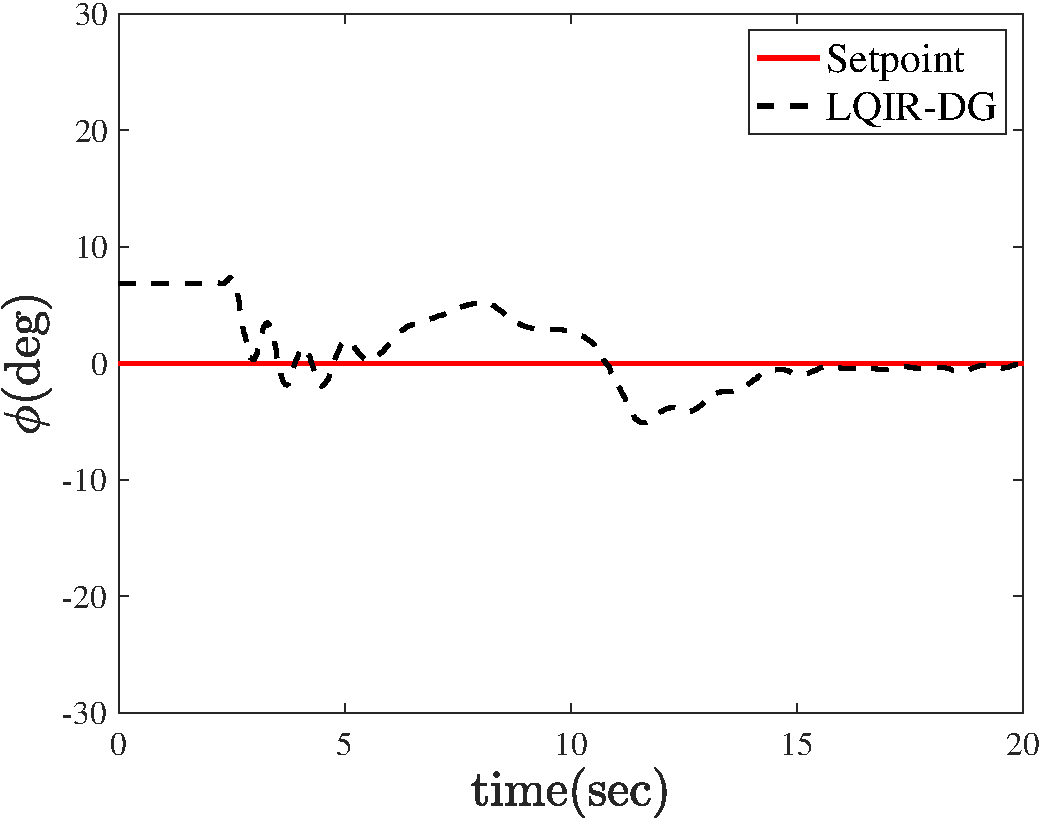
\includegraphics[width=.33\linewidth]{../Figure/implementation/lqidg_roll}}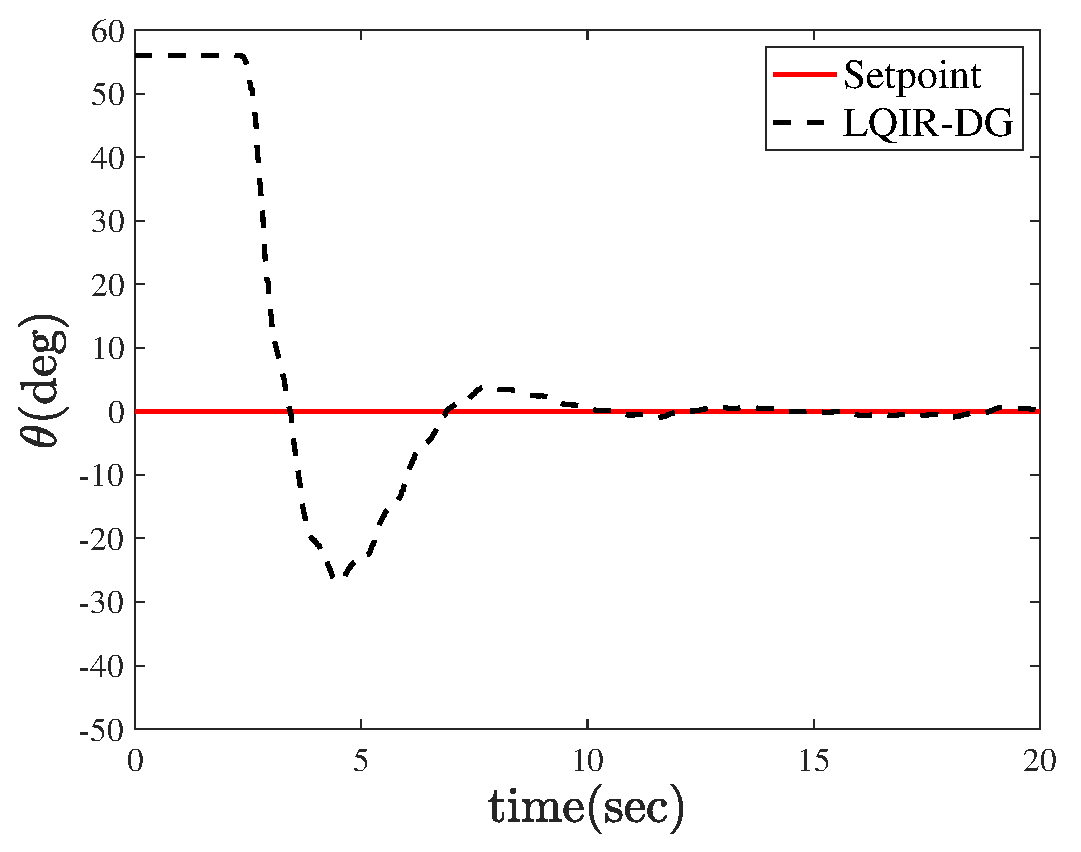
\includegraphics[width=.33\linewidth]{../Figure/implementation/lqidg_pitch}
	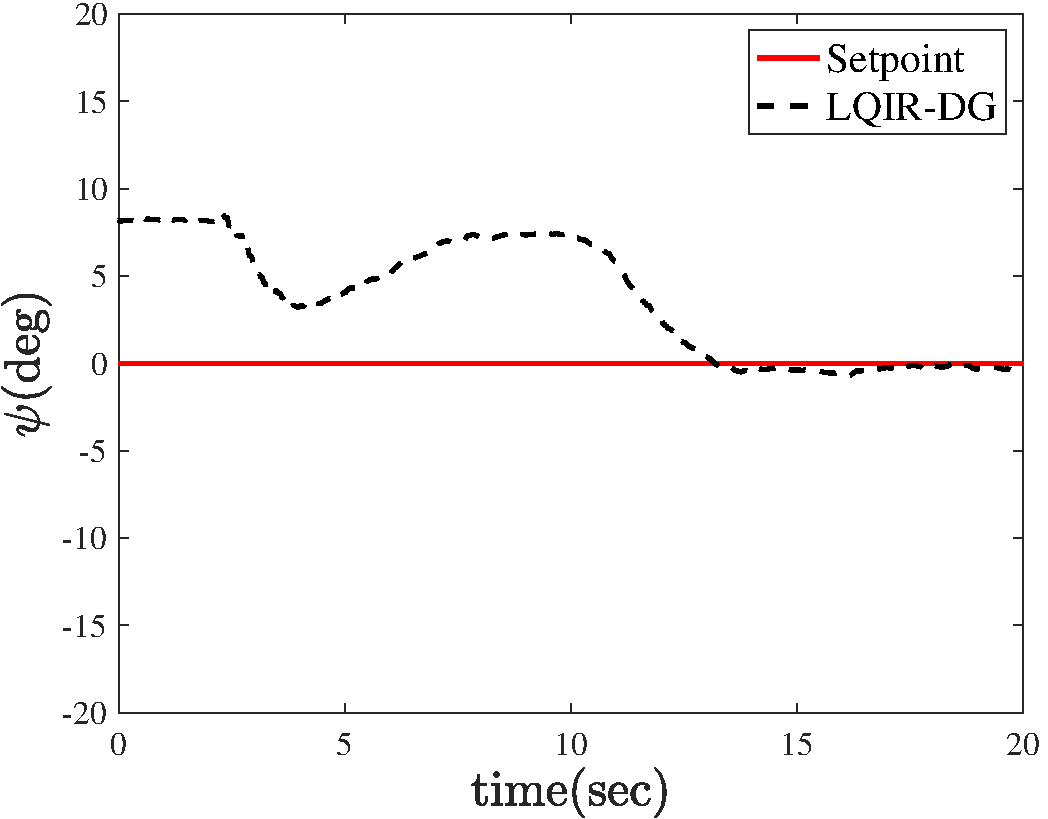
\includegraphics[width=.33\linewidth]{../Figure/implementation/lqidg_yaw}}
	\hfill
	\subfloat[\label{fig:square}]{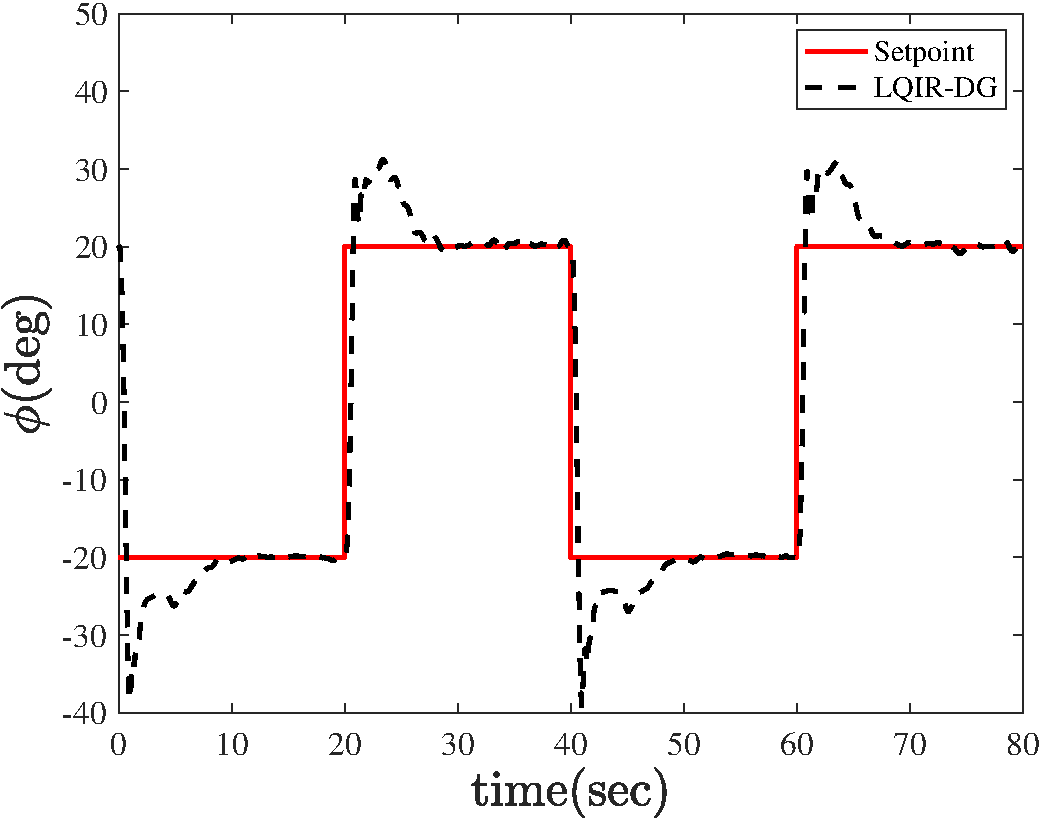
\includegraphics[width=.35\linewidth]{../Figure/implementation/square/lqidg_roll_20}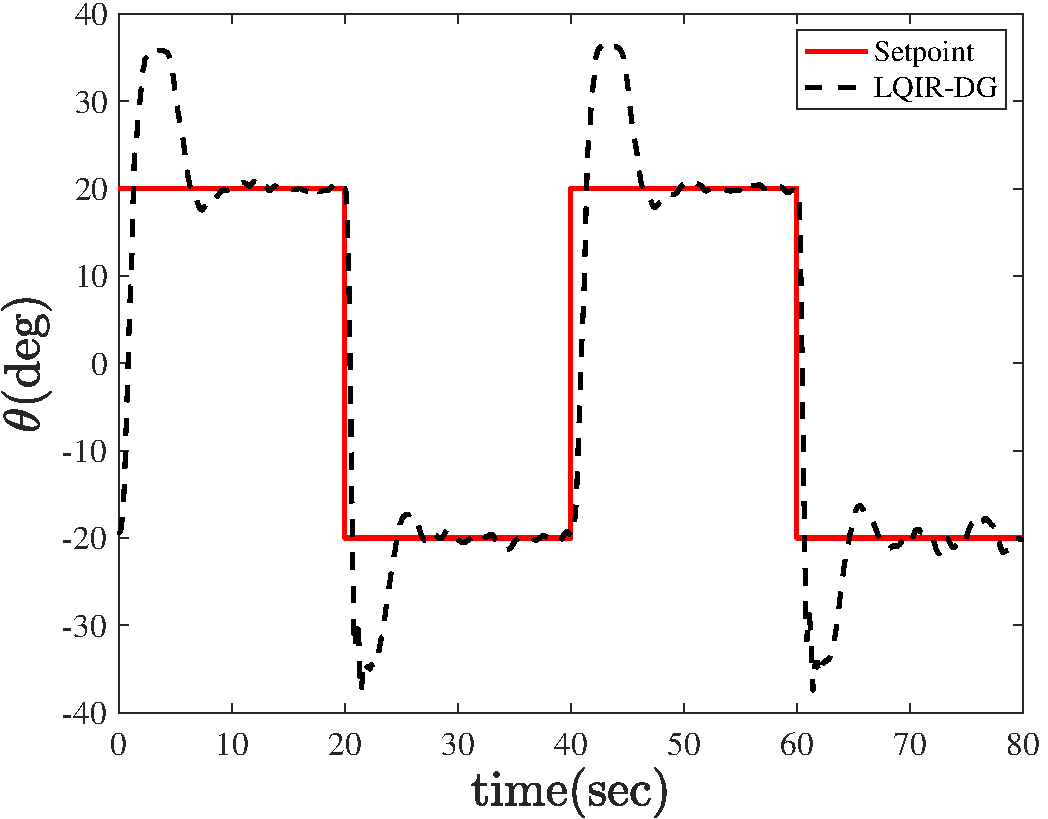
\includegraphics[width=.35\linewidth]{../Figure/implementation/square/lqidg_pitch_20}}
	\caption{Comparison of actual roll and pitch angles with the desired values in \ref{sub@fig:regulation} regulation and \ref{sub@fig:square} tracking problems.}
	\label{fig:result}
\end{figure}

\begin{figure}[H]
	% \vspace{0.3cm}
	\centering
	\subfloat[\label{fig:omega_regulation}]{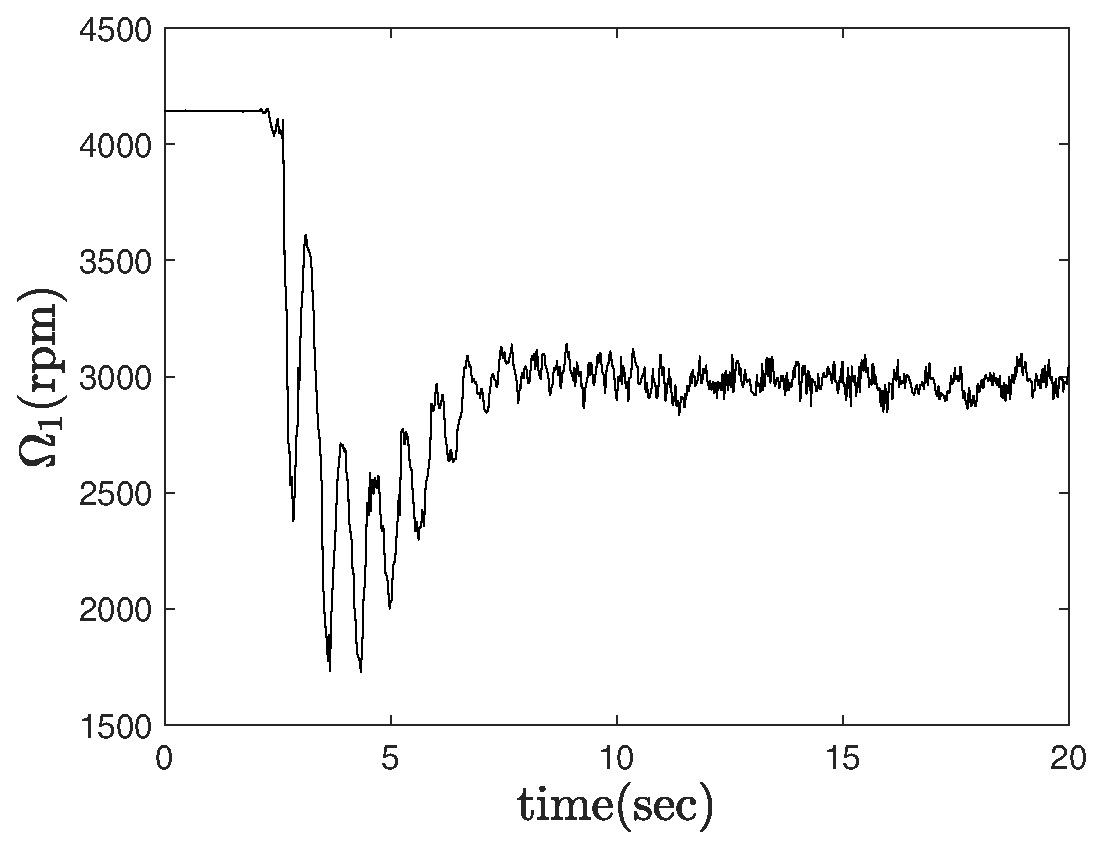
\includegraphics[width=.25\linewidth]{../Figure/implementation/lqidg_Omega_1}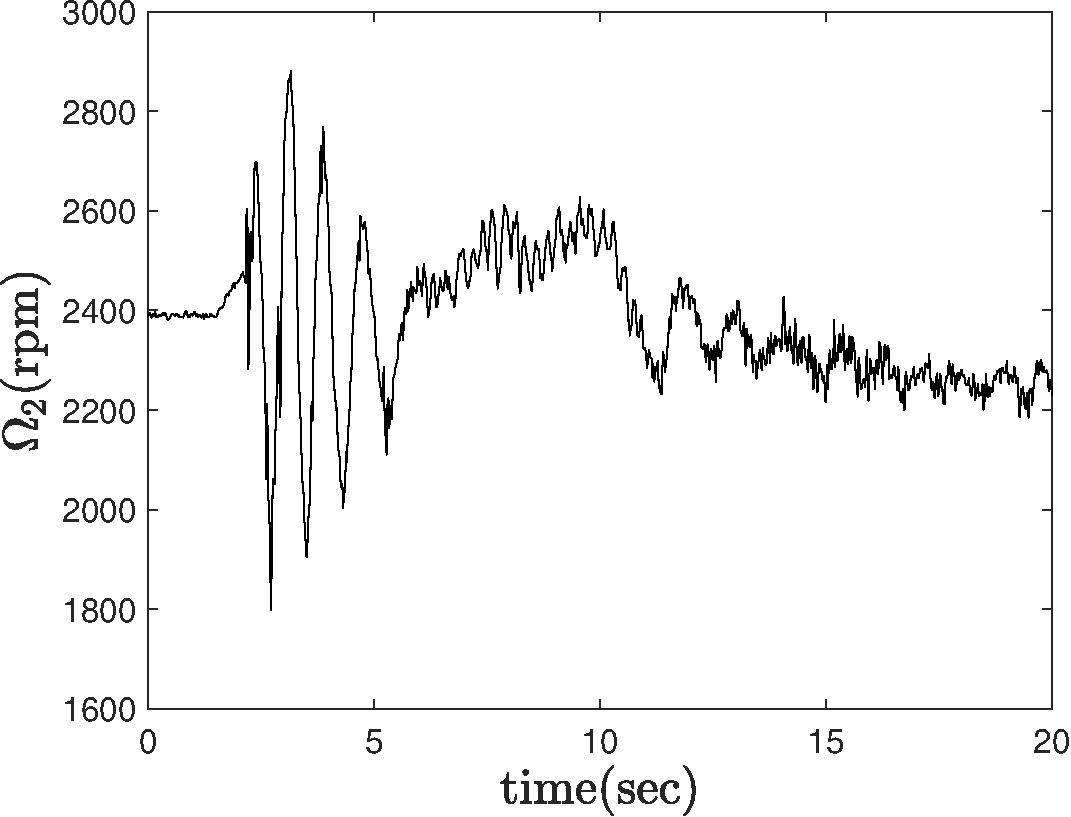
\includegraphics[width=.25\linewidth]{../Figure/implementation/lqidg_Omega_2}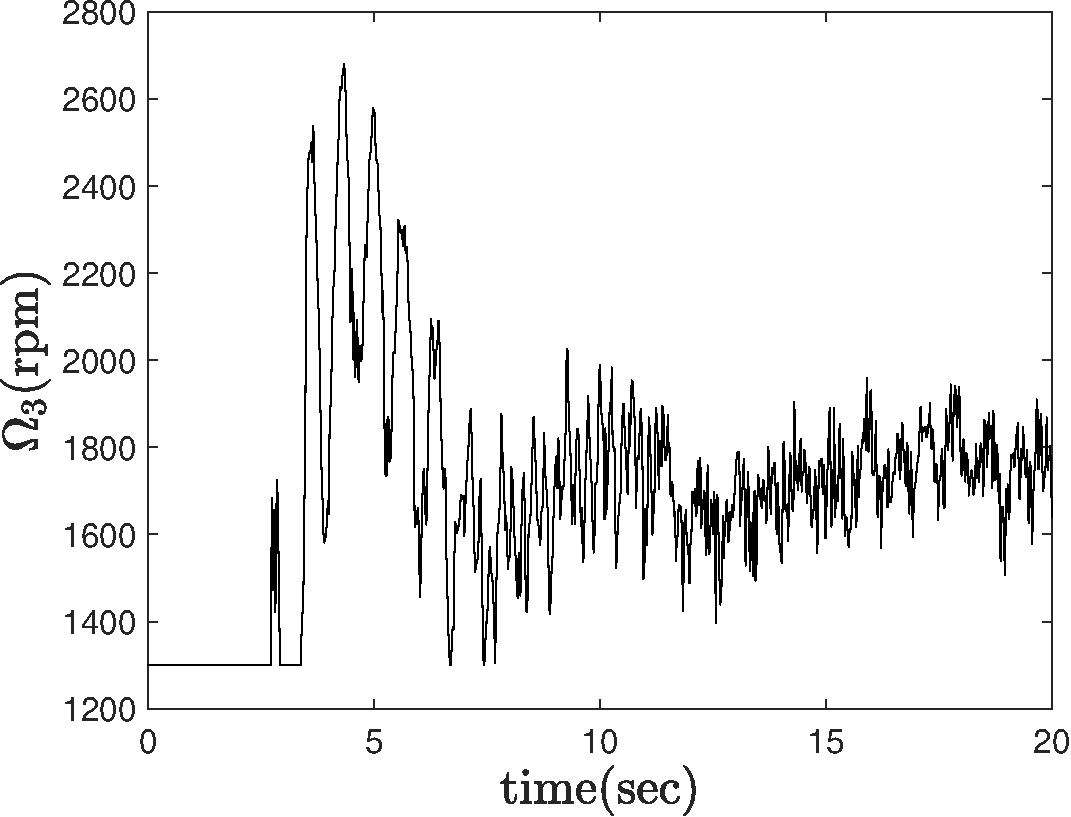
\includegraphics[width=.25\linewidth]{../Figure/implementation/lqidg_Omega_3}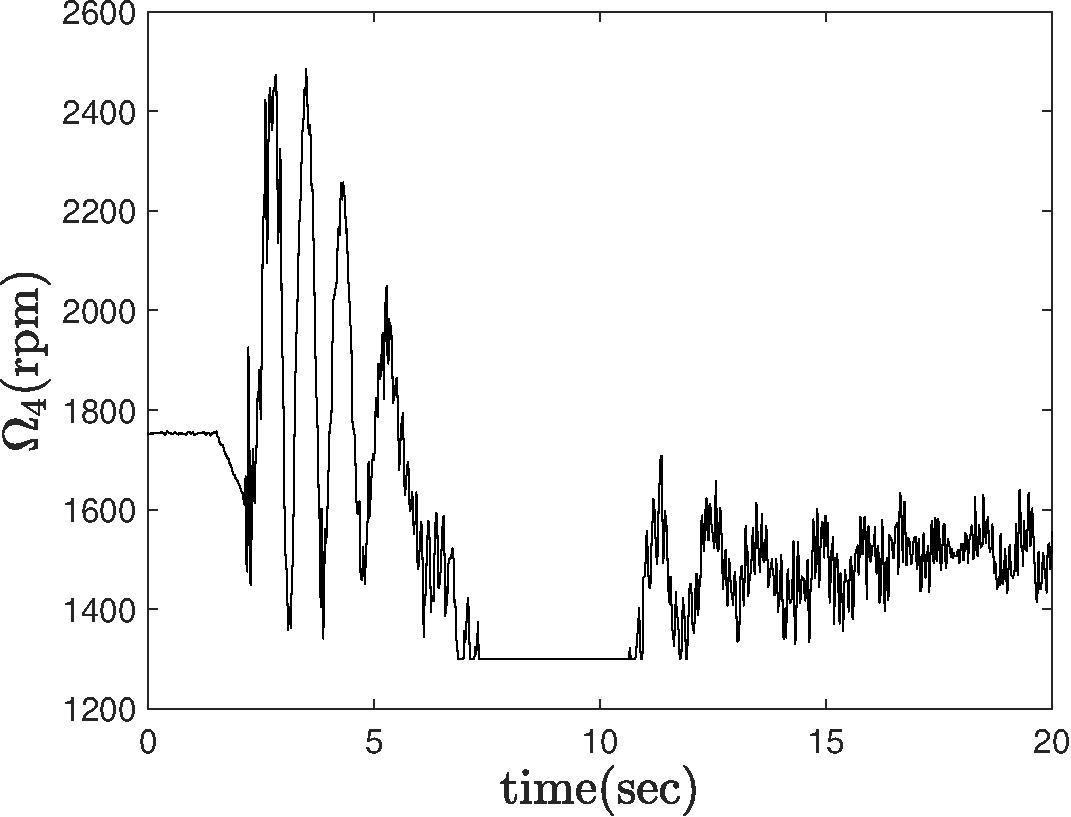
\includegraphics[width=.25\linewidth]{../Figure/implementation/lqidg_Omega_4}
	}
	\hfil
	\subfloat[\label{fig:omega_square}]{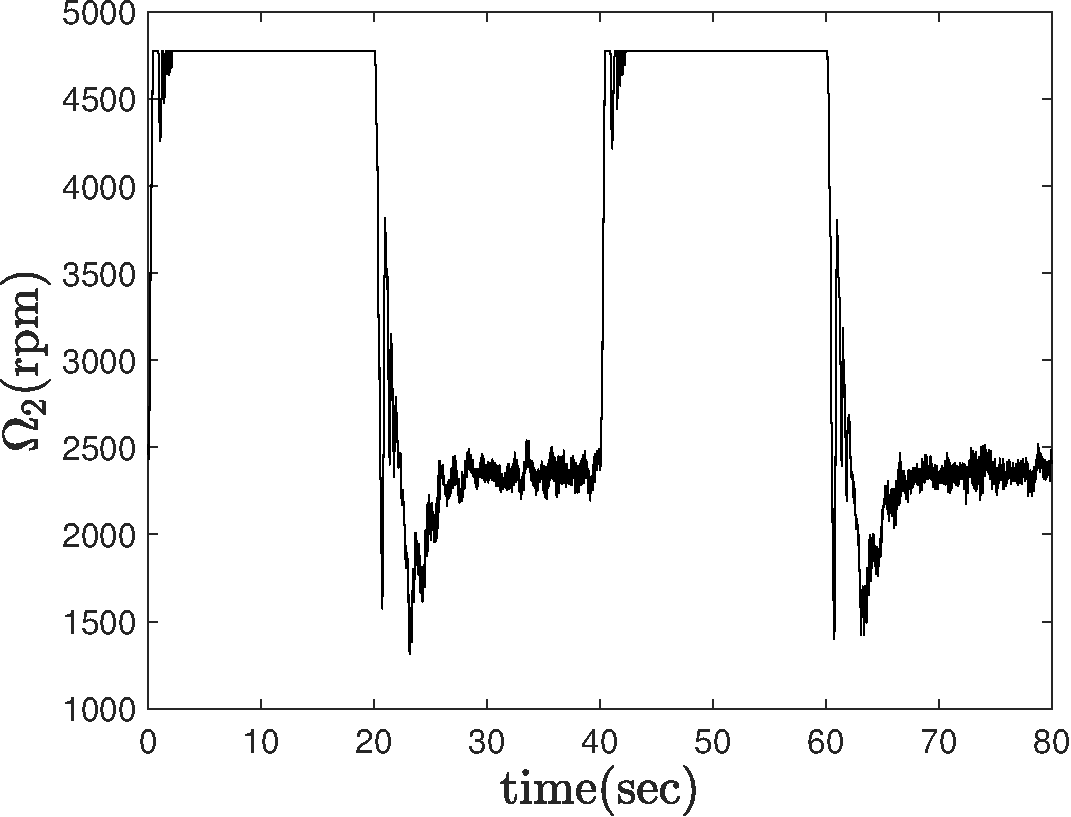
\includegraphics[width=.25\linewidth]{../Figure/implementation/square/lqidg_squre_omega_2}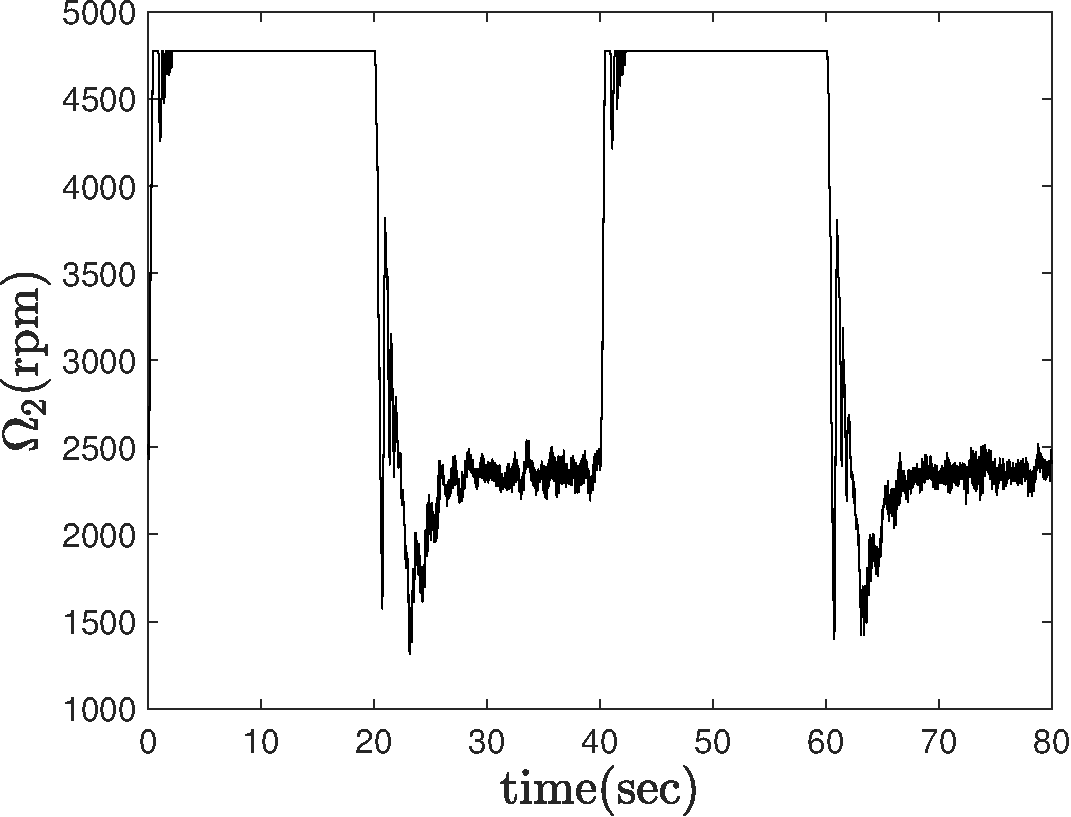
\includegraphics[width=.25\linewidth]{../Figure/implementation/square/lqidg_squre_omega_2}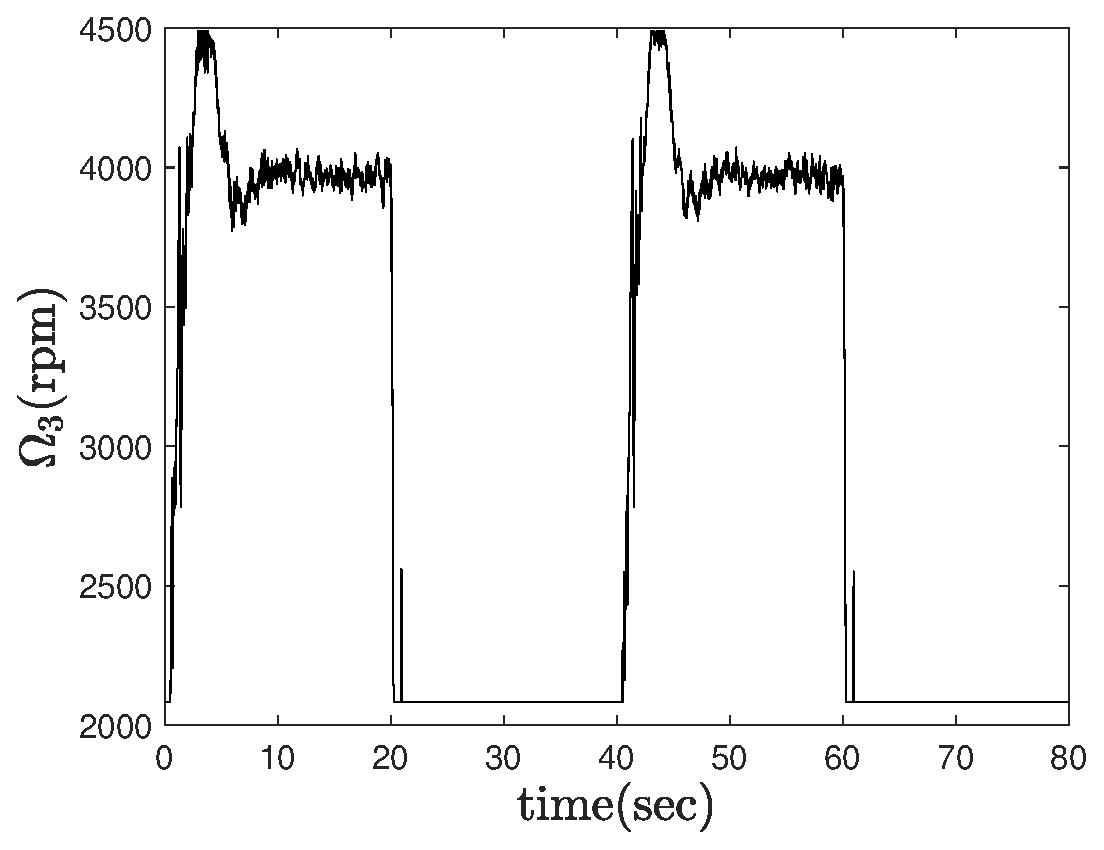
\includegraphics[width=.25\linewidth]{../Figure/implementation/square/lqidg_squre_omega_3}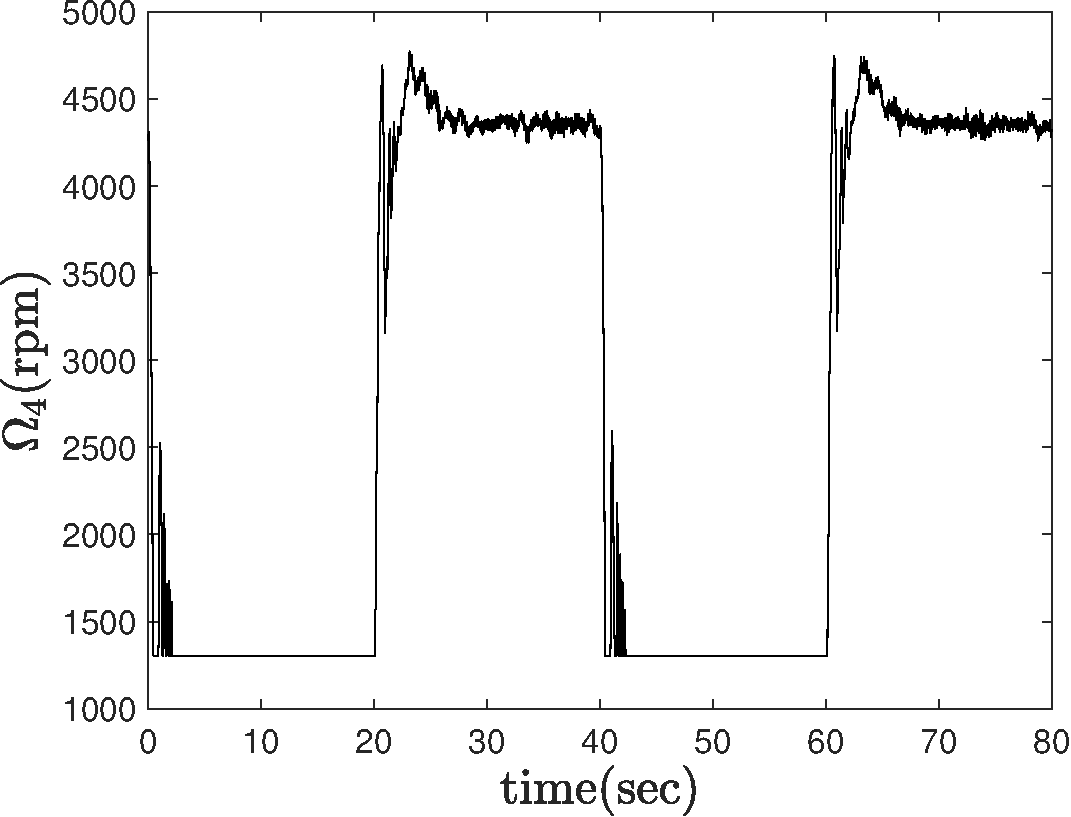
\includegraphics[width=.25\linewidth]{../Figure/implementation/square/lqidg_squre_omega_4}} %%%? didnt describe a and b
	\caption{Rotational velocity  commands in \ref{sub@fig:omega_regulation} regulation and \ref{sub@fig:omega_square} tracking problems.}
	\label{fig:omega}
\end{figure}
\subsubsection{Investigating the Disturbance Rejection}\label{sec:disturbance}
\noindent Here, the effect of the input disturbance is investigated on the performance of the proposed controller.
The input disturbance, $\mathrm{d_{\Omega_i}}$, is considered as a change in the command of the rotational velocity, modeled as %%%? with or in for input disturbace
\begin{equation}
	\mathrm{d_{\Omega_1}} = \mathrm{d_{\Omega_2}} = -\mathrm{d_{\Omega_3}} = -\mathrm{d_{\Omega_4}} = \begin{cases}
		500~{\mathrm{rpm}} \quad &20<t<60\\
		0 \quad &\mathrm{other}
	\end{cases}
\end{equation}
Figure \ref{fig:disturbance} illustrates the roll and pitch angles in the regulation problem, when the input disturbance occurs. These results indicate that the proposed controller can stabilize the quadrotor platform in the presence of input disturbance.



\begin{figure}[H]
	\centering
	\subfloat{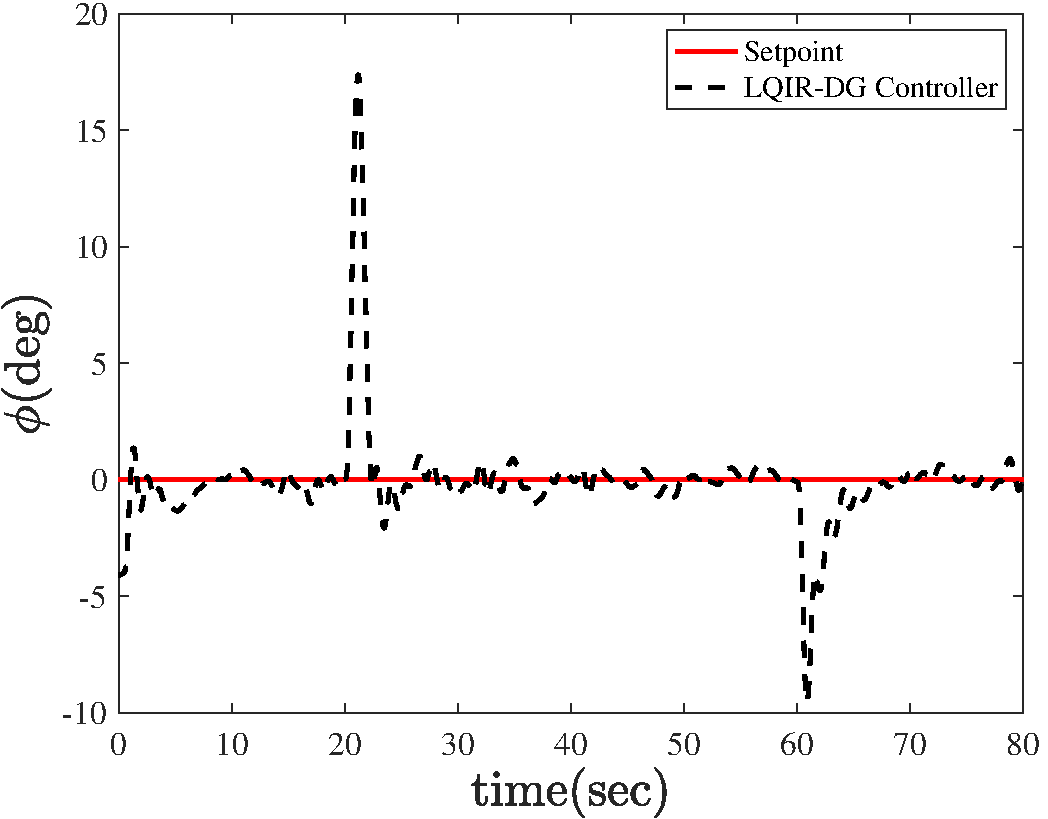
\includegraphics[width=.49\linewidth]{../Figure/implementation/disturbance/lqidg_roll}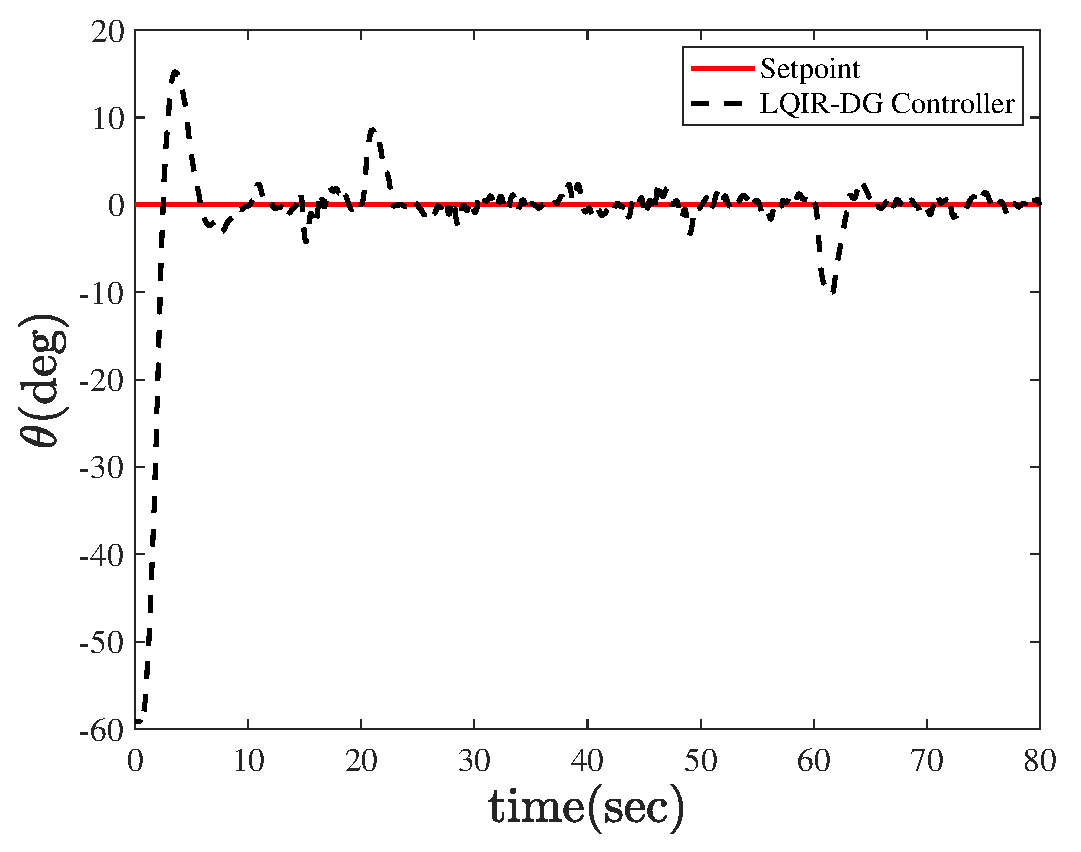
\includegraphics[width=.49\linewidth]{../Figure/implementation/disturbance/lqidg_pitch}
	}
	% \hfill
	% \subfloat[\label{fig:omega_disturbance}]{\includegraphics[width=.23\linewidth]{../Figure/implementation/disturbance/lqidg_Omega_1}\includegraphics[width=.23\linewidth]{../Figure/implementation/disturbance/lqidg_Omega_2}\includegraphics[width=.23\linewidth]{../Figure/implementation/disturbance/lqidg_Omega_3}\includegraphics[width=.23\linewidth]{../Figure/implementation/disturbance/lqidg_Omega_4}}
	
	\caption{Comparison of actual roll and pitch angles with the desired, when the input disturbance occurs.}
	\label{fig:disturbance}
\end{figure}
\subsubsection{Investigating the Impact of Modeling Uncertainty}\label{sec:model-uncertainty}
\noindent The effect of the modeling uncertainty is investigated on the performance of the proposed controller.
To achieve this, 50 and 100 grams weights are added to the roll and pitch axes, respectively, as shown in Figure \ref{fig:quadrotor_with_weight}.
Figure \ref{fig:weight} \ref{sub@fig:weight_roll} compares the desired and the actual roll angle and Figure \ref{fig:weight} \ref{sub@fig:weight_pitch} shows the desired and the actual pitch angle, when the uncertainty of moments of inertia is present.
Moreover, Figure \ref{fig:weight} \ref{sub@fig:omega_weight} shows the rotational velocity commands of the experimental platform, when the model uncertainty is applied.
The implementation results show that the platform outputs converge to the desired values in the presence of the modeling uncertainty.
\begin{figure}[H]
	\centering
	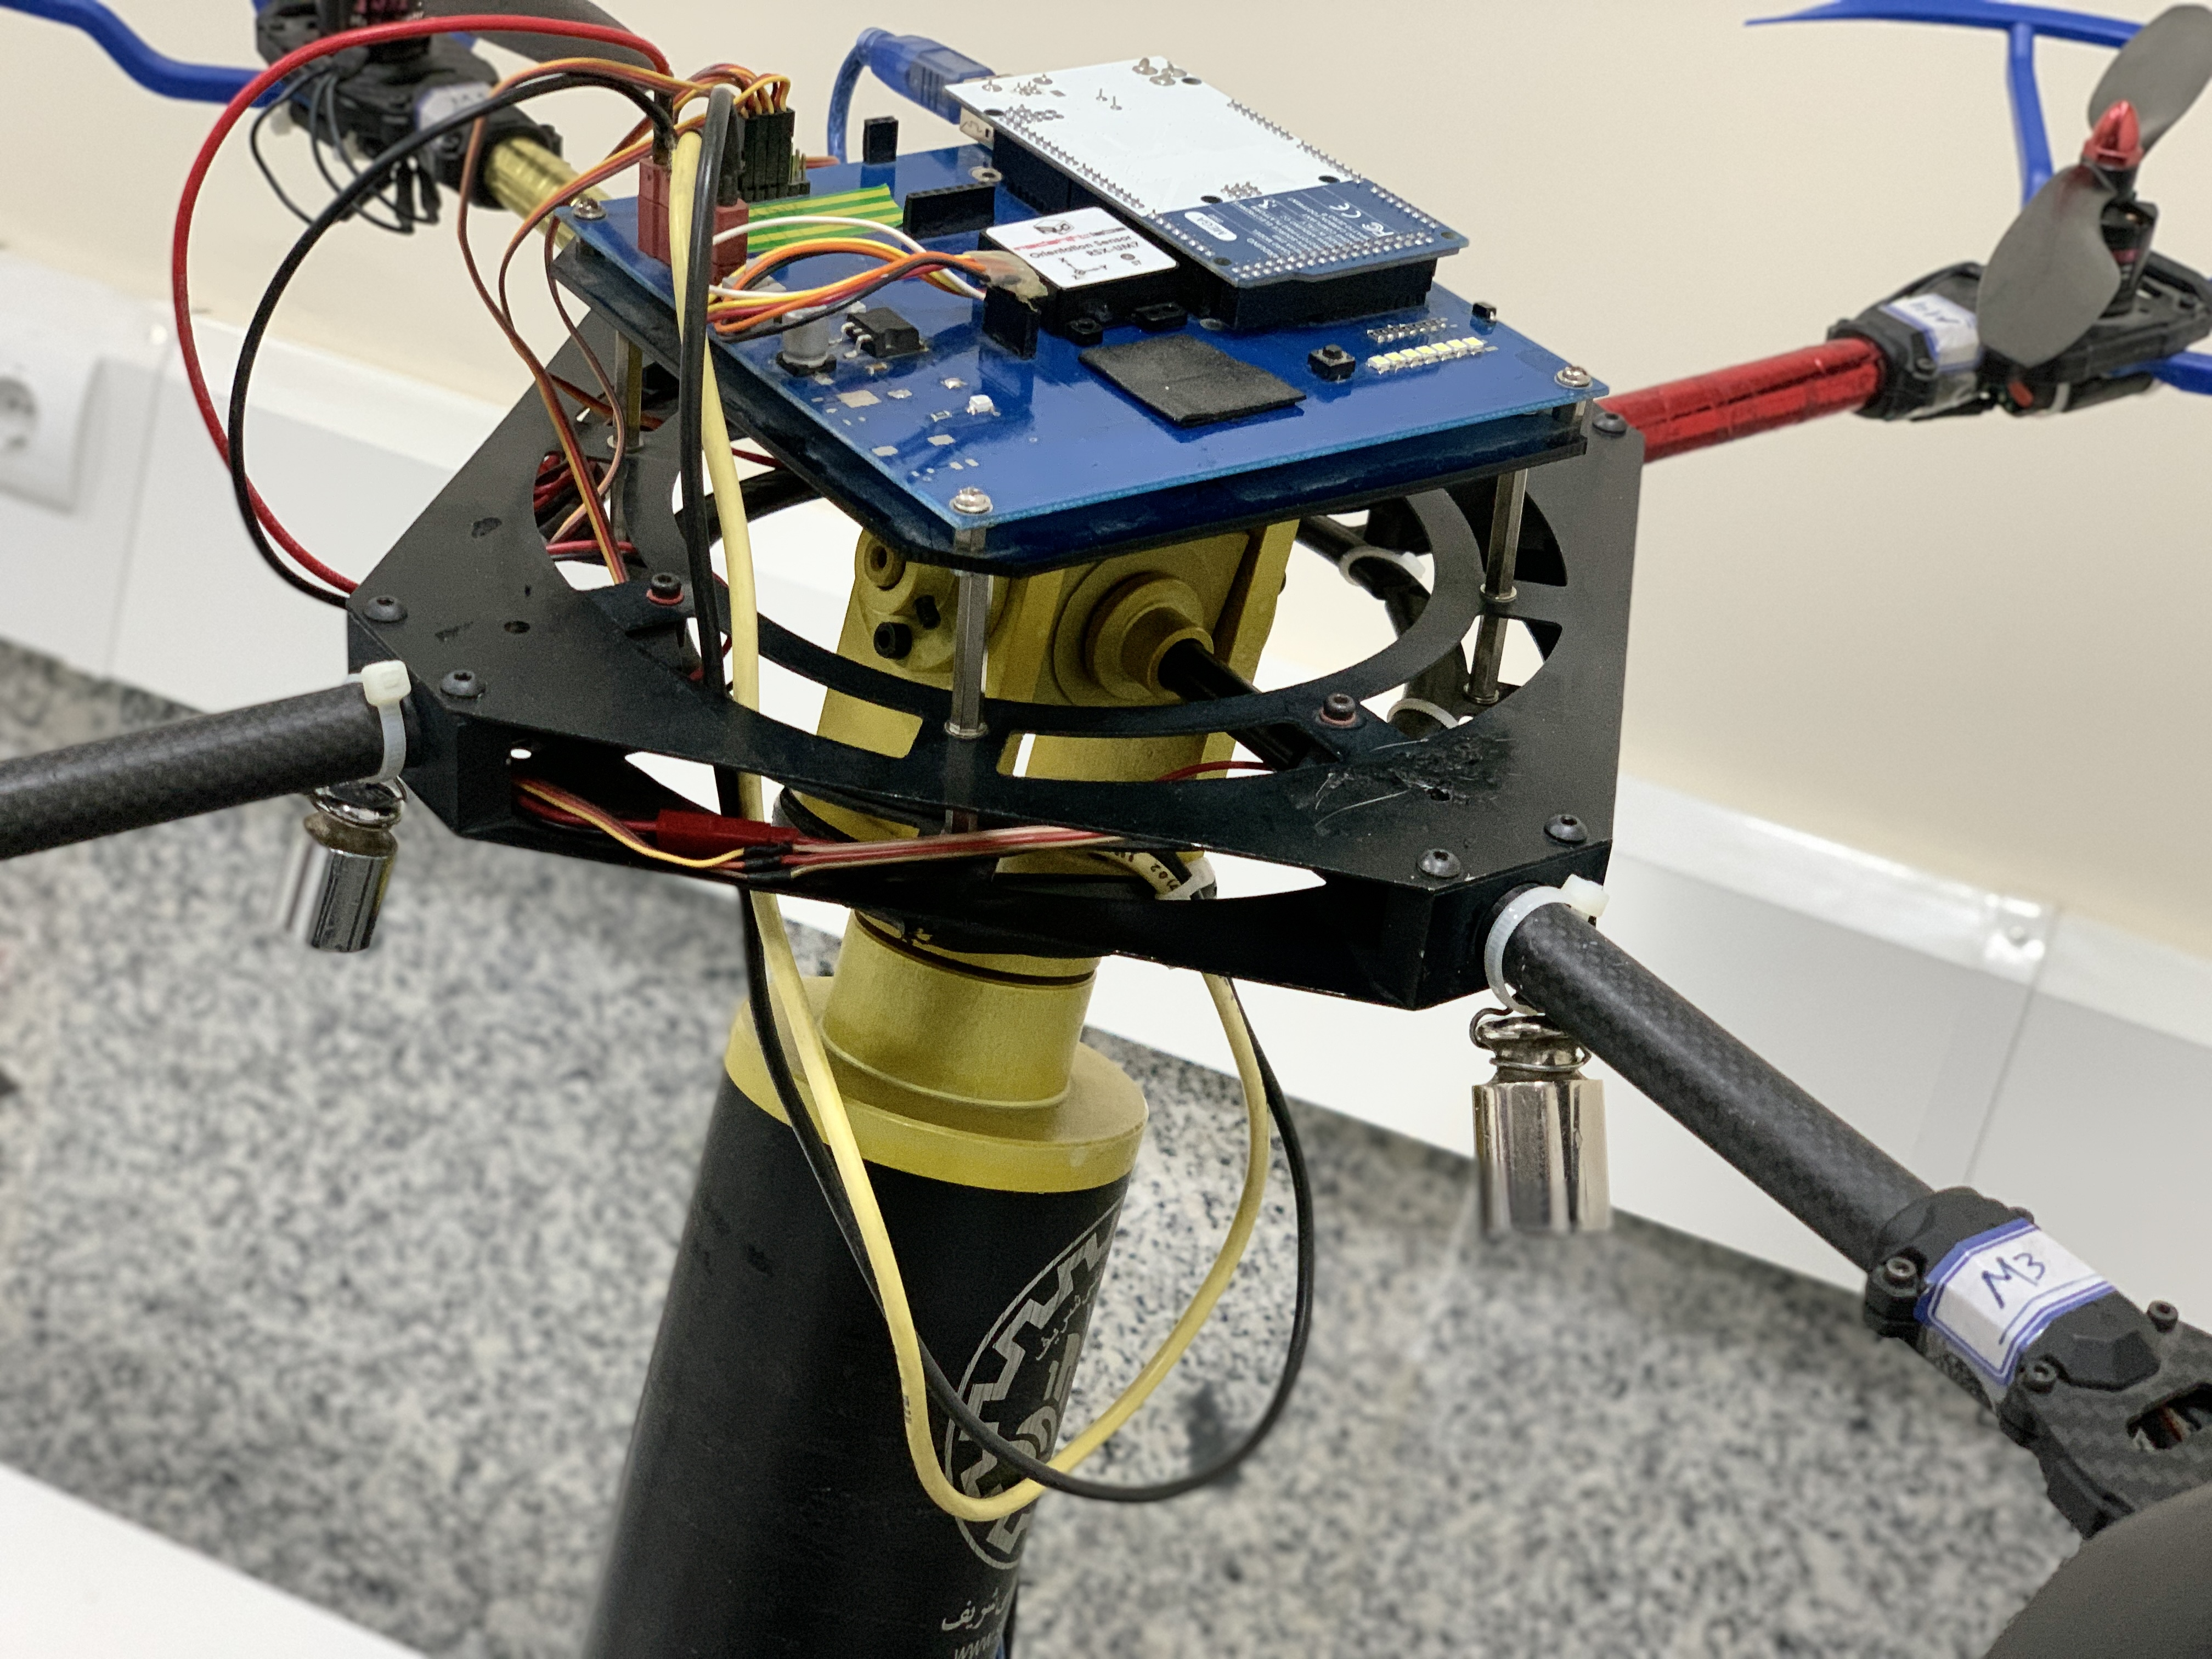
\includegraphics[width=0.45\textwidth]{../Figure/implementation/weight/Quad_with_weight.jpg}
	\caption{Quadrotor 3-DoF platform with added weights.} %%%? is it okey
	\label{fig:quadrotor_with_weight}
%  \end{figure}
%  \begin{figure}[H]
	\centering
	\subfloat[\label{fig:weight_roll}]{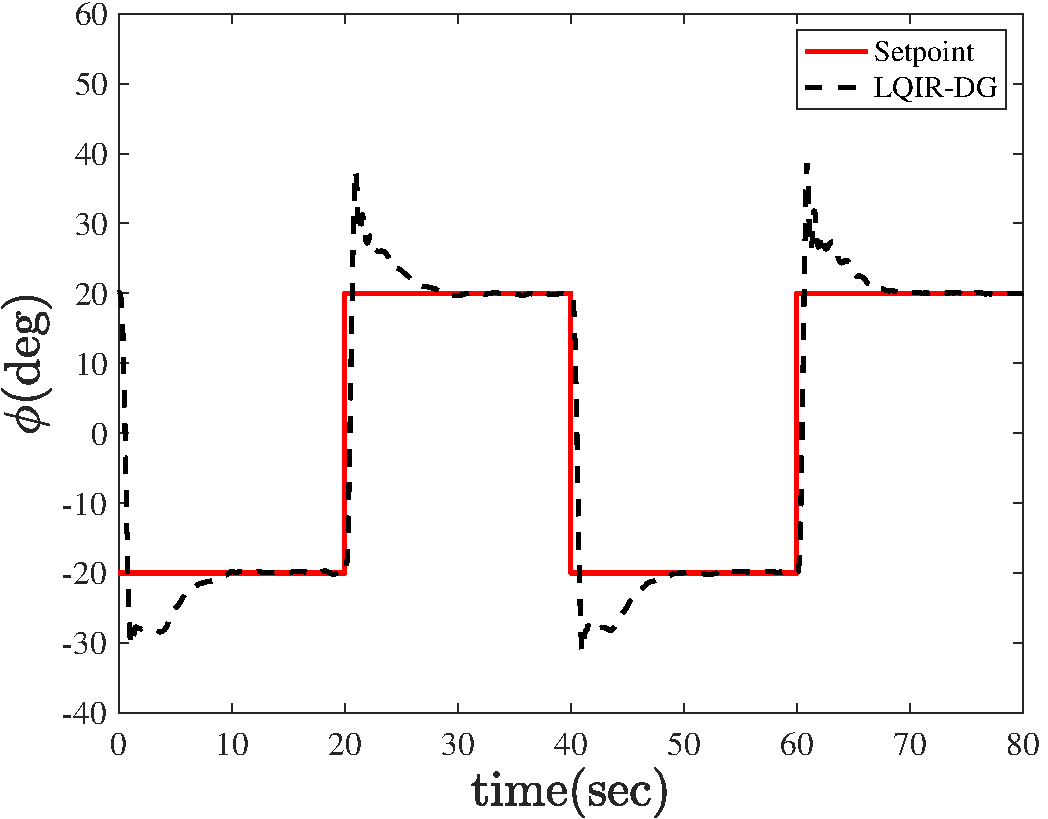
\includegraphics[width=.45\linewidth]{../Figure/implementation/weight/lqidg_roll_20}}\subfloat[\label{fig:weight_pitch}]{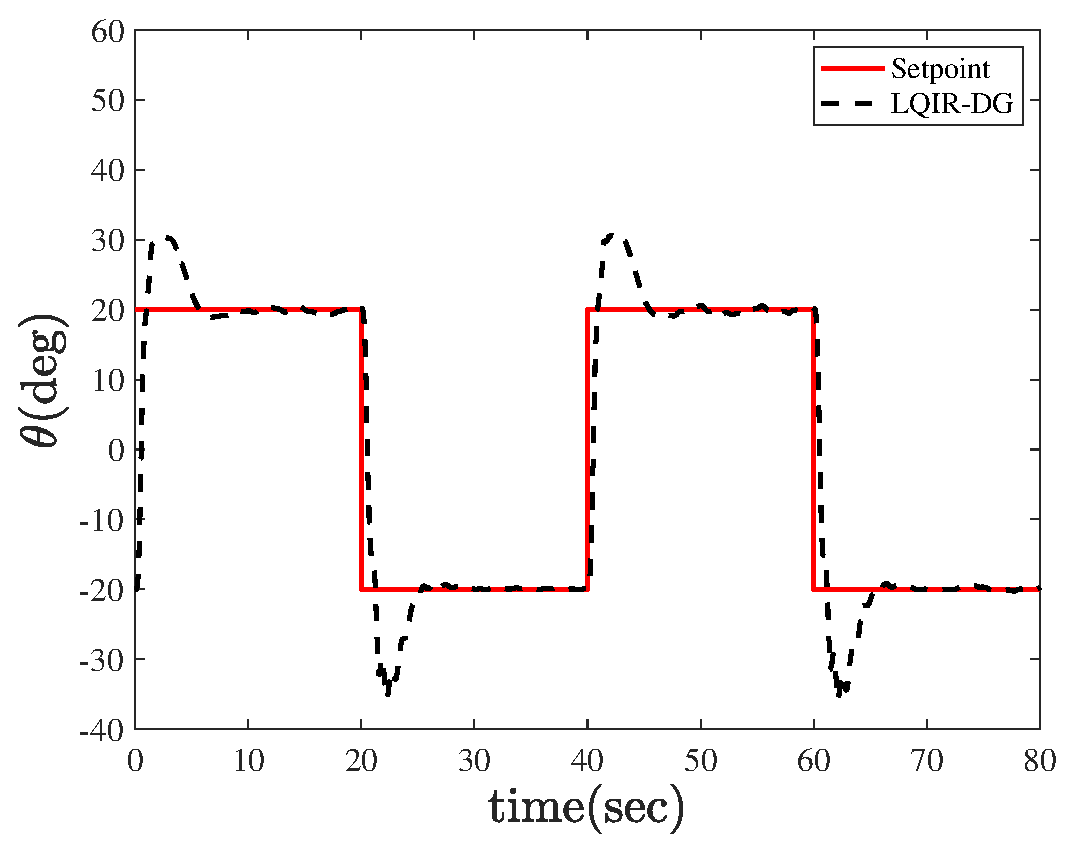
\includegraphics[width=.45\linewidth]{../Figure/implementation/weight/lqidg_pitch_20}
	}
	\hfill
	\subfloat[\label{fig:omega_weight}]{\includegraphics[width=.25\linewidth]{../Figure/implementation/weight/lqidg_Omega_1}\includegraphics[width=.25\linewidth]{../Figure/implementation/weight/lqidg_Omega_2}\includegraphics[width=.25\linewidth]{../Figure/implementation/weight/lqidg_Omega_3}\includegraphics[width=.25\linewidth]{../Figure/implementation/weight/lqidg_Omega_4}}
	\caption{Comparison of actual roll and pitch angles with desired values, when the modeling uncertainty is present.}
	\label{fig:weight}
\end{figure}
\subsubsection{Comparison with the Control Strategies}
\noindent Figure \ref{fig:compare} compares the LQIR-DG controller performance with the PID controller and variant of the LQR strategies such as the LQR and LQIR. 
Moreover, the box plot of all controllers is plotted in Figure \ref{fig:compare_boxplot} for the cost function, introduced in equation \eqref{eq:min_max_cost_function}. %%%? two controller side by side
The median of Root Mean Square Error (RMSE) is shown in the crossline in the box plot.
These results indicate that the proposed controller is able to provide rapid convergence and excellent transient response relative to other controllers for attitude control of the experimental platform.

\begin{figure}[h]
	\centering
	\subfloat[\label{fig:all_roll}]{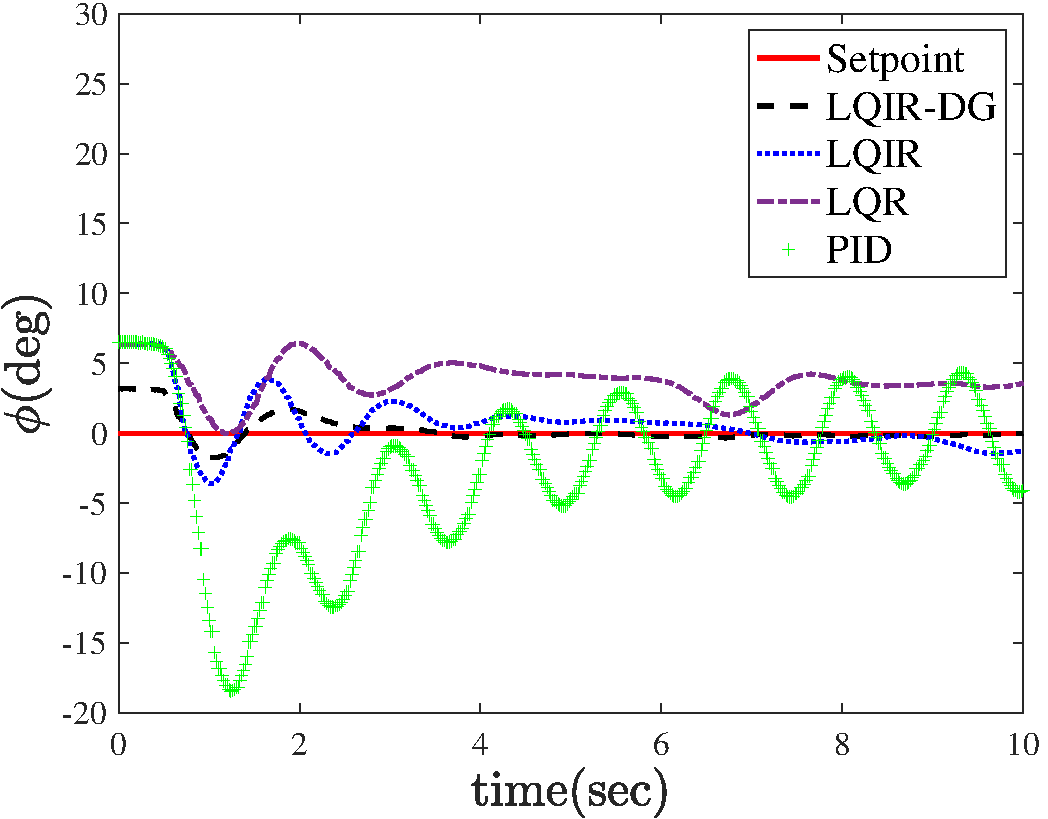
\includegraphics[width=.6\linewidth]{../Figure/implementation/lqidgvslqr/roll}}
	\hfil
	\subfloat[\label{fig:all_pitch}]{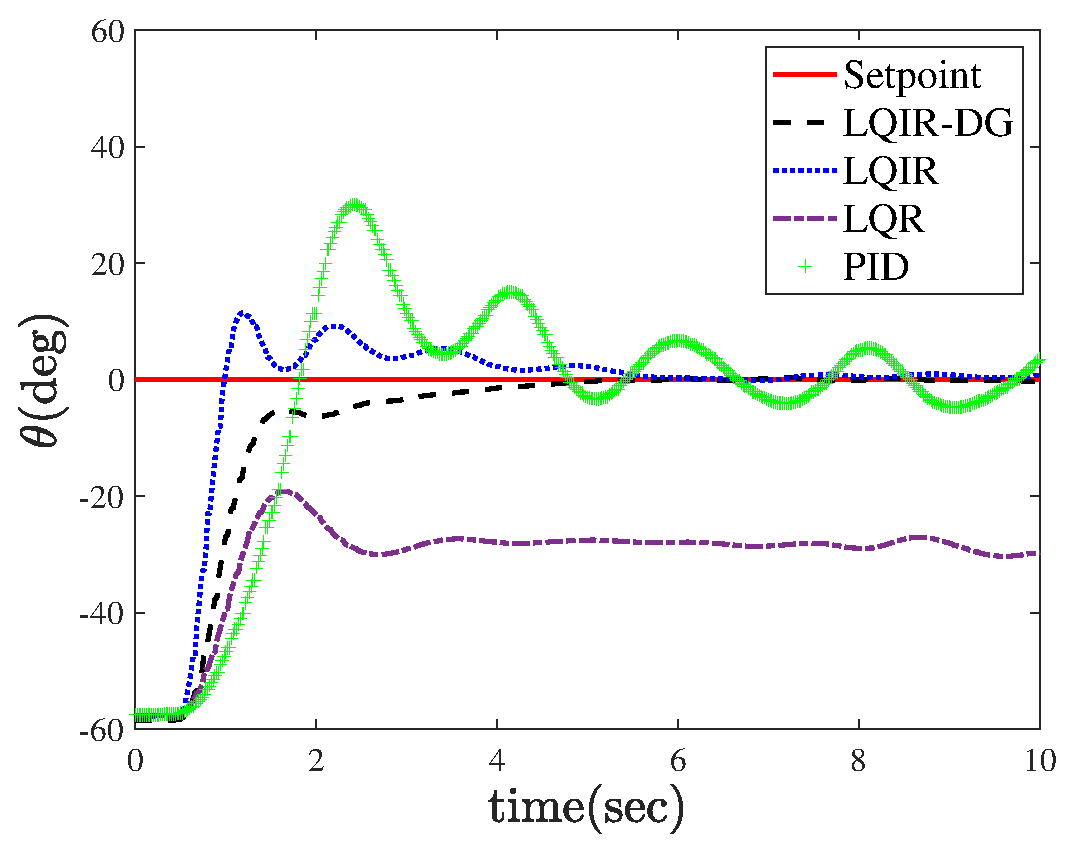
\includegraphics[width=.6\linewidth]{../Figure/implementation/lqidgvslqr/pitch}
	}
	\caption{Comparison of LQIR-DG structure with the variant of LQR and PID in regulation problem: \ref{sub@fig:all_roll} roll angle \ref{sub@fig:all_pitch} pitch angle.}
	\label{fig:compare}
\end{figure}

\begin{figure}[H]
	\centering
	{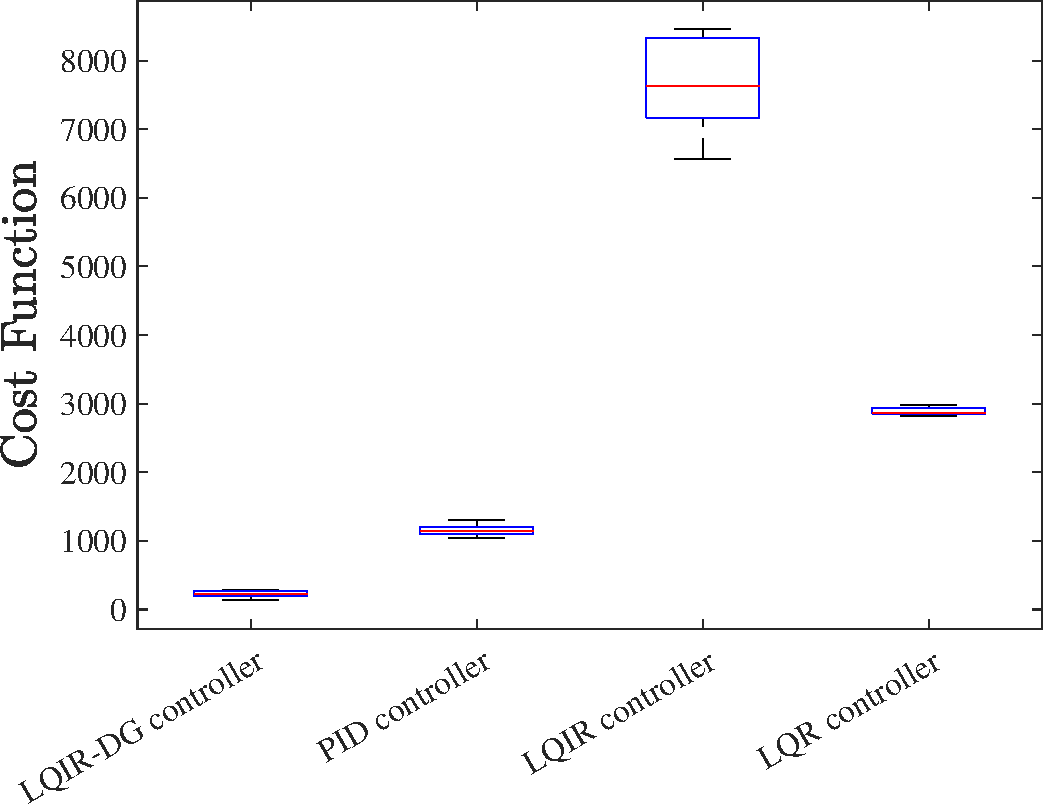
\includegraphics[width=.6\linewidth]{../Figure/implementation/box_plot/lqidgvsboxplot}
	}
	\caption{Box plot of LQIR-DG, LQR, LQIR, and PID controllers.}
	\label{fig:compare_boxplot}
\end{figure}

\section{Conclusion}\label{sec:conclusion}
% \vspace{-0.15cm}
\noindent In this paper, the linear quadratic integral differential game approach, was used in real-time for attitude control of the platform quadrotor. %%%? for quadrotor
For the implementation of the controller structure, an accurate dynamic model was considered for the experimental platform.
Then, the model parameters were identified using the NSL method.
For evaluation of the proposed method, the regulation and tracking  proposed were successfully performed.
Moreover, the ability of the proposed method was investigated in the rejection of the input disturbance and modeling error in the experimental platform.
Finally, a comparison
was also performed between the results of classical PID, LQR, and LQIR with the proposed method.
The implementation results illustrated the excellent performance of the LQIR controller based on the game theory approach in attitude control for the quadrotor platform.



% An example of a floating figure using the graphicx package.
% Note that \label must occur AFTER (or within) \caption.
% For figures, \caption should occur after the \includegraphics.
% Note that IEEEtran v1.7 and later has special internal code that
% is designed to preserve the operation of \label within \caption
% even when the captionsoff option is in effect. However, because
% of issues like this, it may be the safest practice to put all your
% \label just after \caption rather than within \caption{}.
%
% Reminder: the "draftcls" or "draftclsnofoot", not "draft", class
% option should be used if it is desired that the figures are to be
% displayed while in draft mode.
%
%\begin{figure}[!t]
%\centering
%\includegraphics[width=2.5in]{myfigure}
% where an .eps filename suffix will be assumed under latex, 
% and a .pdf suffix will be assumed for pdflatex; or what has been declared
% via \DeclareGraphicsExtensions.
%\caption{Simulation results for the network.}
%\label{fig_sim}
%\end{figure}

% Note that the IEEE typically puts floats only at the top, even when this
% results in a large percentage of a column being occupied by floats.


% An example of a double column floating figure using two subfigures.
% (The subfig.sty package must be loaded for this to work.)
% The subfigure \label commands are set within each subfloat command,
% and the \label for the overall figure must come after \caption.
% \hfil is used as a separator to get equal spacing.
% Watch out that the combined width of all the subfigures on a 
% line do not exceed the text width or a line break will occur.
%
%\begin{figure*}[!t]
%\centering
%\subfloat[Case I]{\includegraphics[width=2.5in]{box}%
%\label{fig_first_case}}
%\hfil
%\subfloat[Case II]{\includegraphics[width=2.5in]{box}%
%\label{fig_second_case}}
%\caption{Simulation results for the network.}
%\label{fig_sim}
%\end{figure*}
%
% Note that often IEEE papers with subfigures do not employ subfigure
% captions (using the optional argument to \subfloat[]), but instead will
% reference/describe all of them (a), (b), etc., within the main caption.
% Be aware that for subfig.sty to generate the (a), (b), etc., subfigure
% labels, the optional argument to \subfloat must be present. If a
% subcaption is not desired, just leave its contents blank,
% e.g., \subfloat[].


% An example of a floating table. Note that, for IEEE style tables, the
% \caption command should come BEFORE the table and, given that table
% captions serve much like titles, are usually capitalized except for words
% such as a, an, and, as, at, but, by, for, in, nor, of, on, or, the, to
% and up, which are usually not capitalized unless they are the first or
% last word of the caption. Table text will default to \footnotesize as
% the IEEE normally uses this smaller font for tables.
% The \label must come after \caption as always.
%
%\begin{table}[!t]
%% increase table row spacing, adjust to taste
%\renewcommand{\arraystretch}{1.3}
% if using array.sty, it might be a good idea to tweak the value of
% \extrarowheight as needed to properly center the text within the cells
%\caption{An Example of a Table}
%\label{table_example}
%\centering
%% Some packages, such as MDW tools, offer better commands for making tables
%% than the plain LaTeX2e tabular which is used here.
%\begin{tabular}{|c||c|}
%\hline
%One & Two\\
%\hline
%Three & Four\\
%\hline
%\end{tabular}
%\end{table}


% Note that the IEEE does not put floats in the very first column
% - or typically anywhere on the first page for that matter. Also,
% in-text middle ("here") positioning is typically not used, but it
% is allowed and encouraged for Computer Society conferences (but
% not Computer Society journals). Most IEEE journals/conferences use
% top floats exclusively. 
% Note that, LaTeX2e, unlike IEEE journals/conferences, places
% footnotes above bottom floats. This can be corrected via the
% \fnbelowfloat command of the stfloats package.




% \section{Conclusion}
% The conclusion goes here.





% if have a single appendix:
%\appendix[Proof of the Zonklar Equations]
% or
%\appendix  % for no appendix heading
% do not use \section anymore after \appendix, only \section*
% is possibly needed

% use appendices with more than one appendix
% then use \section to start each appendix
% you must declare a \section before using any
% \subsection or using \label (\appendices by itself
% starts a section numbered zero.)
%


% \appendices
% \section{Proof of the First Zonklar Equation}
% Appendix one text goes here.

% % you can choose not to have a title for an appendix
% % if you want by leaving the argument blank
% \section{}
% Appendix two text goes here.


% % use section* for acknowledgment
% \section*{Acknowledgment}


% The authors would like to thank...


% Can use something like this to put references on a page
% by themselves when using endfloat and the captionsoff option.
\ifCLASSOPTIONcaptionsoff
  \newpage
\fi



% trigger a \newpage just before the given reference
% number - used to balance the columns on the last page
% adjust value as needed - may need to be readjusted if
% the document is modified later
%\IEEEtriggeratref{8}
% The "triggered" command can be changed if desired:
%\IEEEtriggercmd{\enlargethispage{-5in}}

% references section

% can use a bibliography generated by BibTeX as a .bbl file
% BibTeX documentation can be easily obtained at:
% http://mirror.ctan.org/biblio/bibtex/contrib/doc/
% The IEEEtran BibTeX style support page is at:
% http://www.michaelshell.org/tex/ieeetran/bibtex/
\bibliographystyle{IEEEtran}
% argument is your BibTeX string definitions and bibliography database(s)
\bibliography{bibtex/refs}
%
% <OR> manually copy in the resultant .bbl file
% set second argument of \begin to the number of references
% (used to reserve space for the reference number labels box)
% \begin{thebibliography}{1}

% \bibitem{IEEEhowto:kopka}
% H.~Kopka and P.~W. Daly, \emph{A Guide to \LaTeX}, 3rd~ed.\hskip 1em plus
%   0.5em minus 0.4em\relax Harlow, England: Addison-Wesley, 1999.

% \end{thebibliography}

% biography section
% 
% If you have an EPS/PDF photo (graphicx package needed) extra braces are
% needed around the contents of the optional argument to biography to prevent
% the LaTeX parser from getting confused when it sees the complicated
% \includegraphics command within an optional argument. (You could create
% your own custom macro containing the \includegraphics command to make things
% simpler here.)
%\begin{IEEEbiography}[{\includegraphics[width=1in,height=1.25in,clip,keepaspectratio]{mshell}}]{Michael Shell}
% or if you just want to reserve a space for a photo:

% \vspace{-33pt}
% \begin{IEEEbiography}[{\includegraphics[width=1in,height=1.25in,clip,keepaspectratio]{../Figure/nobahati.jpg}}]{Hadi Nobahari}
% 	received his B.S., M.S., and Ph.D.
% 	in aerospace engineering, flight dynamic, and control
% 	division, from the Sharif University of Technology in
% 	1998, 2000, and 2006, respectively. He is a
% 	Professor in the Department of Aerospace
% 	Engineering of the Sharif University of Technology.
% 	His research interests include novel applications of
% 	heuristic algorithms in aerospace, intelligent guidance
% 	and control systems, cooperative guidance and
% 	navigation systems.
% \end{IEEEbiography}

% % if you will not have a photo at all:
% % \bf{If you include a photo:}
% \vspace{-33pt}
% \begin{IEEEbiography}[{\includegraphics[width=1in,height=1.25in,clip,keepaspectratio]{../Figure/sharifi.jpg}}]{Alireza Sharifi}
% 	was born in Iran in 1988. He
% 	received his M.S. degree in aerospace engineering
% 	from the Sharif University of Technology, Tehran, Iran,
% 	in 2013. He is currently a Ph.D. candidate majored
% 	in aerospace engineering at the Sharif University
% 	of Technology. His research interests are artificial
% 	intelligence, swarm filter, and nonlinear estimation. operative guidance and
% 	 navigation systems.
% \end{IEEEbiography}

% % insert where needed to balance the two columns on the last page with
% % biographies
% %\newpage
% \vspace{-33pt}
% \begin{IEEEbiography}[{\includegraphics[width=1in,height=1.25in,clip,keepaspectratio]{../Figure/baniasad.jpeg}}]{Ali Baniasad}
% 	Ali Baniasad is a highly accomplished aerospace engineer with a passion for intelligent control, optimization, and machine learning.
% 	He received his Bachelor's degree from Sharif University of Technology in 2022, where he excelled in exploring the applications of these techniques in aerospace and robotics systems. 
% 	Ali is currently pursuing a Master's degree at Sharif University, where his research focuses on developing intelligent control systems for autonomous aerial vehicles. 
% 	% With a commitment to advancing the field, Ali aims to make significant contributions to the development of intelligent control and optimization systems in academia and industry.

% % is a highly motivated and accomplished aerospace engineer with a keen interest in intelligent control, optimization, and machine learning. He received his Bachelor's degree in Aerospace Engineering from Sharif University of Technology, Iran, in 2022. During his undergraduate studies, he excelled in his coursework and demonstrated a keen interest in exploring the applications of intelligent control and optimization techniques in aerospace systems.

% % After completing his undergraduate studies, Ali continued to pursue his passion for intelligent control and optimization by gaining hands-on experience in this field. He worked as a research assistant in the Intelligent Control and Robotics Lab at Sharif University, where he was involved in developing novel control algorithms for unmanned aerial vehicles (UAVs) using optimization and machine learning techniques.

% % Ali is currently pursuing Master degree at Sharif University of Technology, where he continues to explore the applications of intelligent control, optimization, and machine learning techniques in robotics. His current research focuses on the development of intelligent control systems for autonomous aerial vehicles, with the aim of enhancing their performance and capabilities in complex environments.

% % With a strong passion for research and a deep commitment to advancing the field of robotics, Ali is dedicated to making significant contributions to the development of intelligent control and optimization systems. He aims to pursue a career in academia and industry, where he can continue to apply his expertise and knowledge to solve complex engineering problems and contribute to the advancement of the field.
% \end{IEEEbiography}

% \vspace{-33pt}
% \begin{IEEEbiography}[{\includegraphics[width=1in,height=1.25in,clip,keepaspectratio]{../Figure/pordal.jpeg}}]{Reza Pordal} received his B.S. degree in aerospace engineering from the Sharif University of Technology in 2021. He is currently pursuing his M.S. degree in aerospace engineering at the Sharif University of Technology. His research interests include multi-agent systems and intelligent control.

% \end{IEEEbiography}



% You can push biographies down or up by placing
% a \vfill before or after them. The appropriate
% use of \vfill depends on what kind of text is
% on the last page and whether or not the columns
% are being equalized.

%\vfill

% Can be used to pull up biographies so that the bottom of the last one
% is flush with the other column.
%\enlargethispage{-5in}



% that's all folks
\end{document}


